\chapter{Experimental Work}
\label{cha:experimental-work}

In this chapter, the defect prediction datasets are first presented and then an example of use of the R \acrlong{fs} packages is given. Finally, an in-depth study of the FSinR package is made where the available algorithms are executed and conclusions are obtained from the results.

\section{Datasets}
\label{sec:datasets}

The chosen datasets have been obtained from an R package of defect prediction datasets for software engineering research called DefectData (\url{https://github.com/klainfo/DefectData}). This package contains 101 defect datasets.

The descriptive statistics of the datasets in this package are:
\begin{itemize}
    \item \textbf{System:} name of the dataset.
    
    \item \textbf{Corpus:} type of data in the dataset. In this case, all of chosen datasets are \acrlong{ck} metrics (\acrshort{ck})\footnote{S.R. Chidamber and C.F. Kemerer proposed a set of metrics known as \acrshort{ck} metrics. Thanks to the measures we can go from an empirical system to a formal system. These metrics are designed to measure the quality of \acrlong{oo} software (\acrshort{oo} software).}.
    
    \item \textbf{Defective Ratio:} percentage of total modules that are defective modules.
        \[\frac{DefectiveModules}{Modules} * 100\]
    
    \item \textbf{Number of Modules:} total modules (instances) of the dataset.
    
    \item \textbf{Number of Defective Modules:} defective modules of the dataset.
    
    \item \textbf{Number of Predictors:} amount of features used in the dataset. In this case, all of them are 20 predictors.
    
    \item \textbf{\acrfull{epv}:} the number of events (defective modules) divided by the number of predictor variables considered in developing the prediction.
        \[\frac{DefectiveModules}{Predictors}\]
\end{itemize}

Six of the total datasets available in this GitHub repository have been selected in order to collect all the relationships in a general way between Defective Ratio and Number of Modules of each dataset. The specific descriptive statistics of the chosen datasets are those shown in Table \ref{tab:descriptive-statistics}.

\begin{table}[H]
\centering
    \begin{tabular}{|c|c|c|c|c|c|c|}
        \hline
        \multirow{3}{*}{\textbf{System}} & \multirow{3}{*}{\textbf{Corpus}} & \multirow{3}{2cm}{\textbf{Defective Ratio}} & \multirow{3}{2cm}{\textbf{Number of Modules}} & \multirow{3}{2cm}{\textbf{Number of Defective Modules}} & \multirow{3}{2cm}{\textbf{Number of Predictors}} & \multirow{3}{*}{\textbf{EPV}} \\
         & & & & & & \\
         & & & & & & \\ \hline
        \textbf{xalan-2.7} & ck & 98.789879 & 909 & 898 & 20 & 44.9000000 \\ \hline
        \textbf{xalan-2.5} & ck & 48.194271 & 803 & 387 & 20 & 19.3500000 \\ \hline
        \textbf{jedit-4.3} & ck & 2.235772 & 492 & 11 & 20 & 0.5500000 \\ \hline
        \textbf{pbeans1} & ck & 76.923077 & 26 & 20 & 20 & 1.0000000 \\ \hline
        \textbf{ckjm} & ck & 50.000000 & 10 & 5 & 20 & 0.250000 \\ \hline
        \textbf{forrest-0.6} & ck & 16.666667 & 6 & 1 & 20 & 0.0500000 \\ \hline
    \end{tabular}
\caption{Descriptive statistics of the chosen datasets.}
\label{tab:descriptive-statistics}
\end{table}

Defective Ratio and Number of Modules are two indicators that collect the most representative descriptive statistics of the chosen datasets since they take into account the number of instances they have, both correct and incorrect, and the percentage of incorrect instances, those that contain defects. Therefore, the datasets have been selected for the following reasons:
\begin{itemize}
    \item \textbf{xalan-2.7:} has a high Defective Ratio and a high Number of Modules.
    \item \textbf{xalan-2.5:} has a medium Defective Ratio and a high Number of Modules.
    \item \textbf{jedit-4.3:} has a low Defective Ratio and a high Number of Modules.
    \item \textbf{pbeans1:} has a high Defective Ratio and a low Number of Modules.
    \item \textbf{ckjm:} has a medium Defective Ratio and a low Number of Modules.
    \item \textbf{forrest-0.6:} has a low Defective Ratio and a low Number of Modules.
\end{itemize}
High number of Modules means that it is one of the datasets with the most modules found in the DefectData package. A low number of Modules means that it is one of the datasets with fewer modules that have been found. After discarding datasets applying the previous restrictions, a high Defect Ratio means that the percentage is greater than 70\%, a medium Defect Ratio is that it is around 50\%, and a low Defect Ratio means that it is less than approximately 30\%.

Table \ref{tab:relationship-datasets} presents in a more summarized and schematic way the chosen datasets and the relationship between Defective Ratio and Number of Modules.

\begin{table}[H]
\centering
    \begin{tabular}{|c|c|c|c|c|}
    \cline{3-5}
    \multicolumn{2}{c|}{} & \multicolumn{3}{c|}{\textbf{Defective Ratio}} \\ \cline{3-5}
    \multicolumn{2}{c|}{} & High & Medium & Low \\ \hline
    \multirow{2}{*}{\textbf{Number of Modules}} & High & \textit{xalan-2.7} & \textit{xalan-2.5} & \textit{jedit-4.3} \\ \cline{2-5}
    & Low & \textit{pbeans1} & \textit{ckjm} & \textit{forrest-0.6} \\ \hline
    \end{tabular}
\caption{Relationship between Defective Ratio and Number of Modules of chosen datasets.}
\label{tab:relationship-datasets}
\end{table}

To configure the DefectData package to use, we first create a vector with the names of all the chosen datasets to make them more readily available. See Listing \ref{cod:dsnames}.

\begin{codefloat}
\begin{lstlisting}[language=R, style=Ccolor]
dsnames <- c("xalan-2.7", "xalan-2.5", "jedit-4.3", "pbeans1", "ckjm", "forrest-0.6")
\end{lstlisting}
\caption{Vector \textit{dsnames} with datasets names.}
\label{cod:dsnames}
\end{codefloat}

The data from the ckjm dataset is loaded to show as an example. To load data from any other dataset, follow these same steps. See Listing \ref{cod:load-data}.
\begin{enumerate}
    \item Load DefectData to access the functions contained in the package with library() command.
    \item Use loadData() function with the name of desired dataset, in this case, ckjm. You have to save the dataset information in a variable to be able to use it later.
    \item Then we can verify that it has been loaded correctly by consulting the values of the dataset variable.
\end{enumerate}

\begin{codefloat}
\begin{lstlisting}[language=R, style=Ccolor]
library(DefectData)
data <- loadData("ckjm")

data$data
data$dep
data$indep
\end{lstlisting}
\caption{Example of load ckjm dataset.}
\label{cod:load-data}
\end{codefloat}

All the datasets in this package are organized in a data.frame as follows. See Figure \ref{fig:dataset-organization}.
\begin{itemize}
    \item \textbf{data:} is another data.frame containing 21 variables (20 features and 1 output feature). These variables are the same in all the chosen datasets, only the number of observations (Number of Modules) changes. In the case of the ckjm dataset, there are 10 observations. To access this data.frame, the name of the variable where the dataset has been stored is used, followed by \$data, in this way data\$data. It can be seen in Listing \ref{cod:load-data}. The data used in these datasets are the \acrshort{ck} metrics and other metrics used for the same purpose, more specifically the metrics are the following \cite{metrics2013}:
    \begin{itemize}
        \item \textbf{\acrshort{wmc}:} This measure is the count of the number of methods in each class. This count also includes Constructors and Destructors of the class. It is an integer.
        
        \item \textbf{\acrshort{dit}:} This count is the maximum length/depth from the node to the root of the tree obtained from the class diagram of the \acrshort{oo} code. It is an integer.
        
        \item \textbf{\acrshort{noc}:} A count of the number of direct children of a given class. It is an integer.
        
        \item \textbf{\acrshort{cbo}:} This metric is a count of the number of other classes to which the current class is coupled, via non-inheritance-related couples. Two classes are coupled when the methods of one class use methods or attributes of another class.  It is an integer.
        
        \item \textbf{\acrshort{rfc}:} It is the count of the set of all methods that can be invoked in response to a message to an object of the class or by some method in the class. It is an integer.
        
        \item \textbf{\acrshort{lcom}:} It counts the number of pairs of methods that do not share attributes. It is an integer.
        
        \item \textbf{\acrshort{ca}:} The number of classes in other packages that depend upon classes within the package is an indicator of the package's responsibility. Each class counts only once. Zero if the package does not contain any classes or if the classes in the package are not used by external classes. It is an integer. 
        
        \item \textbf{\acrshort{ce}:} The number of classes in other packages that the classes in the package depend upon is an indicator of the package's dependence on externalities. It is an integer.
        
        \item \textbf{\acrshort{npm}:} It simply counts all the methods in a class that are declared as public. It can be used to measure the size of an API provided by a package. It is an integer.
        
        \item \textbf{\acrshort{lcom3}:} Number of disjoint components in the graph that represents each method as a node and the sharing of at least one attribute as an edge. It is a numeric (decimal value).
        
        \item \textbf{\acrshort{loc}:} It measures the number of lines in the source code text including blank lines. It is used to know the size of the program. It is an integer.
        
        \item \textbf{\acrshort{dam}:} It is the ratio of the number of private (protected) attributes to the total number of attributes declared in the class. It is a numeric (decimal value).
        
        \item \textbf{\acrshort{moa}:} It is a count of the number of data declarations whose types are user defined classes. It is an integer.
        
        \item \textbf{\acrshort{mfa}:} It is the ratio of the number of methods inherited by a class to the total number of methods accessible by member methods of the class. It is a numeric (decimal value).
        
        \item \textbf{\acrshort{cam}:} This metric captures information about the parameter types of a class's methods. A class is cohesive if all methods of the class use the same set of parameter types. The result can be found between 0 and 1. It is a numeric (decimal value).
        
        \item \textbf{\acrshort{ic}:} It is the number of parent classes to which a given class is coupled. A class is coupled to its parent class if one of its inherited methods is functionally dependent on the new or redefined methods in the class. It is an integer.
        
        \item \textbf{\acrshort{cbm}:} It is the total number of new/redefined methods to which all the inherited methods are coupled. An inherited method is coupled to a new/redefined method if it is functionally dependent on a new/redefined method in the class. This metric is a variant of the \acrshort{ic} metric. It is an integer.
        
        \item \textbf{\acrshort{amc}:} It is the average method size for each class. Pure virtual methods and inherited methods are not counted. The assumption behind this metric is that a large method, containing more code, tends to introduce more bugs than a small method. It is a numeric (decimal value).
        
        \item \textbf{MAX\_\acrshort{cc}:} It is the maximum of the McCabe's \acrfull{cc}. McCabe's \acrlong{cc} is equal to the number of different paths to execute a method plus one.
            \[CC = paths + 1\]
        It can also be calculated as number of edges in the graph minus number of nodes of the graph plus number of connected components (connectors).
            \[CC = edges - nodes + connectors\]
        It is an integer.
        
        \item \textbf{AVG\_\acrshort{cc}:} It is the average of the McCabe's \acrlong{cc}. It is a numeric (decimal value).
        
        \item \textbf{bug:} It is the output value and means if this module, instance or observation has an error. If it has an error, the value is TRUE and if it does not, it is FALSE. It is a logical value.
    \end{itemize}
    
    \item \textbf{dep:} contains a variable of type character string with the name of the dependent feature on the others, that is, the output feature. In the chosen datasets, the output function is always "bug". As above, the value is queried using data\$dep as seen in Listing \ref{cod:load-data}.
    
    \item \textbf{indep:} is a vector of characters with the rest of the features being independent. In the chosen datasets, there are always the same 20 features. This information is queried using data\$indep as in Listing \ref{cod:load-data}. It outputs the vector with the name of all the features excluding the dependent feature.
\end{itemize}

\begin{figure}[H]
    \centering
    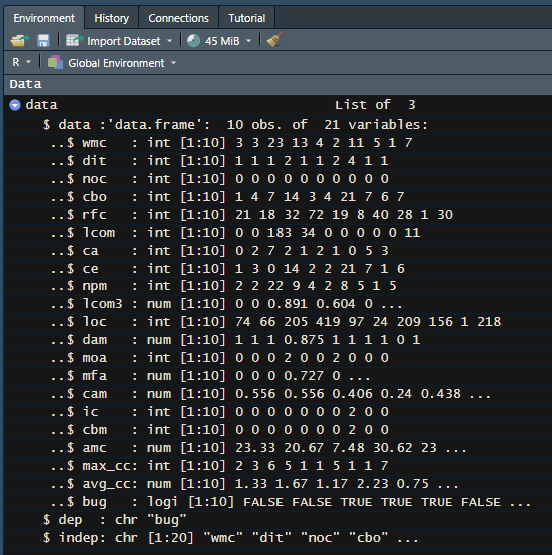
\includegraphics[scale=2]{dataset-organization.png}
    \caption{Image of RStudio Environment with dataset organization.}
    \label{fig:dataset-organization}
\end{figure}

To make it easier to load a dataset, a function has been created that performs all of the above steps. In the same script, the vector with the name of the chosen datasets is added for better future access. See Listing \ref{cod:loadDataset.R}.

\begin{codefloat}[H]
\lstinputlisting[language=R, style=Ccolor]{listings/loadDataset.R}
\caption{loadDataset.R script.}
\label{cod:loadDataset.R}
\end{codefloat}

To make use of the function or the vector it is necessary to load the script with the source() \footnote{source() causes R to accept input from the named file. The entire file is read and parsed, then the parsed expressions are added to the environment.} function and the path of the script as a parameter. Then the loadDataset() function can be called with the parameter of the name of the dataset to be loaded. To consult the vector, you just have to write the name of the variable where it is stored, dsnames. See an example in Listing \ref{cod:loadDataset-use}.

\begin{codefloat}[H]
\begin{lstlisting}[language=R, style=Ccolor]
source("./loadDataset.R")
dsnames
loadDataset("ckjm")
\end{lstlisting}
\caption{Example of loadDataset.R use.}
\label{cod:loadDataset-use}
\end{codefloat}

\section{R Packages for FS}
\label{sec:r-packages-fs}

The \acrfull{cran} is a network of servers that stores a wide variety of multipurpose packages with R code and documentation. R is designed to calculate statistics and create graphs.The \acrlong{fs} is part of the more complex concept that is statistics. It also makes use of statistical metrics in its procedures.

In this section, five R packages that are used to perform \acrshort{fs} are going to be explained and tested. Of course, they are not the only ones that \acrshort{cran} makes available for open use, but they are very representative and help to understand in a fairly simple way how the selection of attributes is carried out.

\subsection{FSinR Package}
\label{sec:fsinr-package}

This package contains many different filter and wrapper methods that are combined with search algorithms to get the best subset of features. Once the results of the chosen method, filter or wrapper have been obtained, the search algorithm helps to select the evaluated subsets by guiding the process in the feature space \cite{fsinr}.

Functions from the \acrshort{caret} package \cite{caret} can also be used for train the models training to increase the number of possibilities and functionalities. The package is intuitive and very easy to use because it has a main method for the \acrshort{fs} process.

We will now show a basic demonstration of the use of the FSinR package. The functions of the package that are going to be needed are the following.

\textbf{featureSelection} is the main function of the package. It performs the feature selection process. Given a search algorithm and an evaluation method, it uses the search algorithm in combination with the evaluation results to guide the feature selection process to an optimal subset. The arguments of this function are:

\begin{itemize}
    \item \textbf{data:} a matrix or data.frame with the dataset where the observations are in the rows and the features and the target variable are in the columns.
    
    \item \textbf{class:} the name of the dependent variable.
    
    \item \textbf{searcher:} the algorithm to guide the search in the feature space.
    
    \item \textbf{evaluator:} the evaluation method to obtain a measure of the features. The evaluation method can be a filter or a wrapper method.
\end{itemize}

This function returns a list with the results of the feature selection process. The most important item on the list is \textbf{bestFeatures}, a vector with all features where selected features are marked with 1 and unselected features are marked with 0. The list also contains other information such as the evaluation measure (bestValue), evaluation type (evaluationType), evaluation method used (evaluationMethod), type of evaluation measure (measureType), search method used (searchMethod), if the objective of the process is to minimize or maximize the evaluation measure (target), number of features (numFeatures), name of the features (xNames), name of the dependent variable (yNames) and the user time, system time, and total time of the feature selection process (time).

\textbf{searchAlgorithm} is the function which allows to select the search algorithm to be used in the feature selection process. It generates a search function. This function can be run separately to perform a search process in the feature space, but in this case, it is passed as a parameter to the featureSelection function in the searcher parameter. The arguments of this function are:

\begin{itemize}
    \item \textbf{searcher:} name of the search algorithm. The available search algorithms are:
    
    \begin{itemize}
        \item sequentialForwardSelection: \acrfull{sfs}.
        \item sequentialFloatingForwardSelection: \acrfull{sffs}
        \item sequentialBackwardSelection: \acrfull{sbs}
        \item sequentialFloatingBackwardSelection: \acrfull{sfbs}
        \item breadthFirst: Breadth first search
        \item deepFirst: Deep first search
        \item geneticAlgorithm: \acrfull{ga}
        \item whaleOptimization: \acrfull{woa}
        \item antColony: \acrfull{aco}
        \item simulatedAnnealing: \acrfull{sa}
        \item tabu: \acrfull{ts}
        \item hillClimbing: \acrfull{hc}
        \item LasVegas: \acrfull{lv}
    \end{itemize}
    
    \item \textbf{params:} a list of specific parameters to the search method. It depends if the chosen searcher needs to be called with parameters or not. By default it is an empty list.
\end{itemize}

This function returns the chosen search function.

\textbf{filterEvaluator} is the function which allows to select a filter method. It generates a filter function to be used as an evaluator in the feature selection process. This function can also be run directly to generate an evaluation measure. In this case, it will be used to pass it as the evaluator parameter to the featureSelection function. The arguments of this function are:

\begin{itemize}
    \item \textbf{filter:} name of the filter method. The available filter methods are:
    
    \begin{itemize}
        \item binaryConsistency: Binary consistency measure.
        \item chiSquared: Chi squared measure.
        \item cramer: Cramer V measure.
        \item determinationCoefficient: R Squared, to continous features.
        \item fscore: F-score measure.
        \item gainRatio: The gain ratio measure.
        \item giniIndex: Gini index measure.
        \item IEConsistency: Inconsistent Examples consistency measure.
        \item IEPConsistency: Inconsistent Examples Pairs consistency measure.
        \item Jd: Jd evaluation measure.
        \item MDLC: \acrshort{mdlc} evaluation measure.
        \item mutualInformation: The mutual information measure.
        \item roughsetConsistency: Rough Set consistency measure.
        \item relief: Relief.
        \item ReliefFeatureSetMeasure: Relief Feature Set Measure evaluation measure.
        \item symmetricalUncertain: Symmetrical uncertain measure.
    \end{itemize}
    
    \item \textbf{params:} a list of specific parameters to the filter method. It depends if the chosen filter needs to be called with parameters or not. By default it is an empty list.
\end{itemize}

This function returns a filter method that is used to generate an evaluation measure.

As said before, the FSinR package allows the possibility of using the 238 models available in the \acrshort{caret} package as wrapper methods. The \textbf{wrapperEvaluator} function has the same use as the filterEvaluator function; it sets set all parameters of these methods and generate the wrapper model. It can be used both as an evaluator parameter and alone.

It is important to know that in this package there is a wrapperEvaluator function for wrapper methods, but in this case we will focus on filter methods. There are several reasons. The wrapperEvaluator function is intended to use the functions of the \acrshort{caret} package, but the purpose of this section is to study the FSinR package. The operation of the \acrshort{caret} package will be explained in the \ref{sec:caret-package} section. On the other hand, filter methods are faster than wrapper methods since they do not involve model training and, therefore, are computationally simpler.

Now it will explain how the package works. It is important to note that the FSinR package does not divide data into training and test data. Instead, it applies the feature selection process to the entire dataset passed to it as a parameter. The steps to follow are those:

\begin{enumerate}
    \item First, the filter method must be generated. This is done with the function \textbf{filterEvaluator}.

    In this case, according to "How to Choose a Feature Selection Method For Machine Learning" article \cite{fs-method-ml}, we know that the chosen dataset has a numerical input and a categorical output (logic). According to the article "How to Perform Feature Selection With Numerical Input Data" \cite{fs-numerical}, there are two popular feature selection techniques that can be used for numerical input data and a categorical (class) target variable: ANOVA-f Statistic and Mutual Information Statistics. The mutual information measure is one of the filters that are already implemented in the FSinR package but the input data should be discrete and it's not. Coefficient of determination or R Squared measure is similar to an ANOVA (analysis of variance) measure. Both methods find the "line of best fit" that minimizes the sum-of-squared residuals, and calculate the residual variance as a fraction of the total unconditional variance of the outcome. Therefore, \textbf{determinationCoefficient} is the chosen method.
    
    \item The next step is to generate the search algorithm. This is done by calling the \textbf{searchAlgorithm} function and specifying the algorithm you want to use. Section \ref{sec:measures-fsinr} executes each of the search algorithms available in this package to calculate its stability and complexity.
    
    \item Once we have generated the search algorithm and the filter method we call the main function, \textbf{featureSelection}, that performs the feature selection process. Store the result in a variable.
    
    \item Finally, the results show the best subset of features found. The information obtained can be consulted with the name of the variable where the result of \acrshort{fs} has been saved followed by \textbf{\$bestFeatures}.
\end{enumerate}

To make it easier to apply the FSinR package to all the datasets chosen in Section \ref{sec:datasets}, a function has been created that collects the steps explained. The function has been saved in an R script so that it can be used later in Section \ref{sec:measures-fsinr}. Listing \ref{cod:applyFSinR.R} shows the source code for the function.

\begin{codefloat}[H]
\lstinputlisting[language=R, style=Ccolor]{listings/applyFSinR.R}
\caption{applyFSinR.R script.}
\label{cod:applyFSinR.R}
\end{codefloat}

\textbf{applyFSinR} function has two parameters:

\begin{itemize}
    \item \textbf{dsname:} name of the dataset on which the \acrshort{fs} is going to be applied.
    
    \item \textbf{algorithm:} name of search algorithm to be used from those that are available.
\end{itemize}

The code is developed as follows:

\begin{itemize}
    \item First it loads FSinR package and loadDataset.R script.
    
    \item Then it gets the data from dataset using loadDataset function (Listing \ref{cod:loadDataset.R}) and dsname as parameter.
    
    \item Create the evaluator with filterEvaluator function and determinationCoefficient as parameter.
    
    \item Create the searcher with searchAlgorithm. It depends of the input parameter called algorithm.
    
    \item Finally, featureSelection runs. The dependent variable is bug.
\end{itemize}

applyFSinR function returns a list with the best features checked. The features marked with 1 means that it has been selected and 0 that it has not.

\subsection{Boruta Package}
\label{sec:boruta-package}

Boruta is a \acrshort{fs} method. As has been explained throughout this project, that means judging which of the features are important and which are not. It is not like the FSinR package explained in the Section \ref{sec:fsinr-package}, Boruta is the name of the package and an algorithm too.

Under the hood, Boruta algorithm \cite{Boruta} uses feature importance scores which are provided by certain machine learning methods, in particular Random Forest. This algorithm is a wrapper built around the random forest classification algorithm implemented in the R package randomForest \cite{randomForest}. The random forest classification algorithm is relatively quick, can usually be run without tuning of parameters and it gives a numerical estimate of the feature importance.

Boruta package does not contain a large number of functions as it focuses on the use of a single algorithm. The basic functions necessary to carry out a simple example of \acrshort{fs} will be explained.

\textbf{Boruta} function is the main function of the package. It implements the mentioned algorithm. It is capable of working with any classification method that generates a \acrfull{vim}. Boruta uses a top-down search for relevant features. It compares the importance of original features with a random calculated importance of feature copies (shadows). Then it removes irrelevant features to stabilise that test. For a basic use of the Boruta function, it is necessary to know three arguments:

\begin{itemize}
    \item \textbf{x:} it specifies the model using a formula or a data frame of predictors.
    
    \item \textbf{data:} it is the input parameter for dataset in which to interpret formula.
    
    \item \textbf{doTrace:} tracking level of the steps performed by the algorithm. It can be put from level 0 to 3 with the meaning:
    
    \begin{enumerate}
        \setcounter{enumi}{-1}
        \item means no tracing.
        \item means reporting decision about each attribute as soon as it is justified.
        \item means the same as 1 plus reporting each importance source run.
        \item  means the same as 2, plus reporting of hits assigned to yet undecided attributes.
    \end{enumerate}
\end{itemize}

This function returns an object of class Boruta with different components such as a factor of Confirmed, Rejected and Tentative values with the final result (finalDecision), a data frame of importances in each source run (ImpHistory), time taken by the computation (timeTaken), the source of importance (impSource) and the original call of the Boruta function (call).

\textbf{print} function is a method for the Boruta object. The argument of this function is:

\begin{itemize}
    \item \textbf{x:} an object of a class Boruta.
\end{itemize}

This function returns a small description of the results of the execution of the Boruta function. It reports the number of iterations, time of execution, important attributes, unimportant attributes and tentative attributes.

\textbf{plot} function is a default plot method for Boruta objects, showing boxplots of attribute importances over run. For a basic execution of plot function, it is necessary to know one argument:

\begin{itemize}
    \item \textbf{x:} an object of a class Boruta.
\end{itemize}

This function returns an image of boxplots. Blue boxplots correspond to minimal, average
and maximum Z score (Boruta importance measure) of a shadow feature. Red and green boxplots represent Z scores of respectively rejected and confirmed features.

\textbf{plotImpHistory} function is an alternative plot method for Boruta objects, showing matplot of attribute importances over run. For a basic execution, it is necessary to know one argument:

\begin{itemize}
    \item \textbf{x:} an object of a class Boruta.
\end{itemize}

This function returns an image of a graph that shows the importance of each attribute during the iterations performed (classifier run).

\textbf{getSelectedAttributes} function extracts the names of the selected attributes. The arguments of this function are:

\begin{itemize}
    \item \textbf{x:} an object of a class Boruta, from which relevant attributes names should be extracted.
    
    \item \textbf{withTentative:} if set to TRUE, Tentative attributes will be also returned. It is FALSE by default.
\end{itemize}

This function returns a vector of names of attributes selected during a Boruta run.

Knowing now the basic functions to understand how to make \acrshort{fs} with the Boruta package, an example of how it works will be shown. The code sequence to follow is shown in Listing \ref{cod:boruta-use}.

\begin{codefloat}[H]
\begin{lstlisting}[language=R, style=Ccolor]
source("loadDataset.R")
data <- loadDataset("ckjm")

library(Boruta)
set.seed(1)

results <- Boruta(bug~., data = data, doTrace = 2)

print(results)
plot(results)
plotImpHistory(results)

selected <- getSelectedAttributes(results)
\end{lstlisting}
\caption{Example of Boruta package use.}
\label{cod:boruta-use}
\end{codefloat}

The code follows these steps:

\begin{enumerate}
    \item First we use the function loadDataset (Listing \ref{cod:loadDataset.R}) to get the data from the ckjm dataset. We can use all available datasets from the DefectData package but this has been chosen for the examples. See Table \ref{tab:descriptive-statistics} to remember ckjm dataset characteristics.
    
    \item We need to load Boruta package to use it. A fixed seed is then established. This is done since the Boruta algorithm uses randomness. Setting a seed in R means initializing a pseudorandom number generator. When using functions that sample pseudo-random numbers, each time you execute it you will get a different result. The code is not reproducible because the seed that R used to generate that sequence is not known. In this case, it is interesting that each time it is executed, the same results come out in order to make a better observation of them. To set a seed, simply use the set.seed function with an integer as a parameter that will be the same in all executions.
    
    \item Now we can run Boruta function. As first parameter, the model formula is entered in the form "bug\~{ }." where bug is the dependent variable and the point includes the rest of the dataset columns (independent variables). Second parameter means that the data variable is the one that provides the data for the algorithm and third means that it will report on the decision on each attribute as soon as it is justified and on each execution of source of importance.
    
    \item The output of print execution is shown in Listing \ref{cod:print-output}.
    
\begin{codefloat}[H]
\begin{lstlisting}[language=R, style=console]
Boruta performed 99 iterations in 1.458832 secs.
 1 attributes confirmed important: npm;
 16 attributes confirmed unimportant: amc, avg_cc, ca, cbm, cbo and 11 more;
 3 tentative attributes left: cam, loc, wmc;
\end{lstlisting}
\caption{print output.}
\label{cod:print-output}
\end{codefloat}

    \item The output of plot execution is shown in Figure \ref{fig:boxplot}.
    
    \begin{figure}[H]
        \centering
        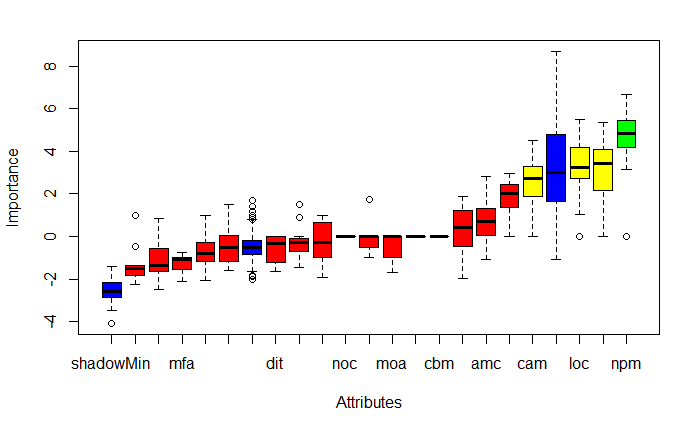
\includegraphics[scale=0.8]{boxplot.png}
        \caption{Boxplots of feature importances over run.}
        \label{fig:boxplot}
    \end{figure}
    
    \item The output of plotImpHistory execution is shown in Figure \ref{fig:graphic}.
    
    \begin{figure}[ht]
        \centering
        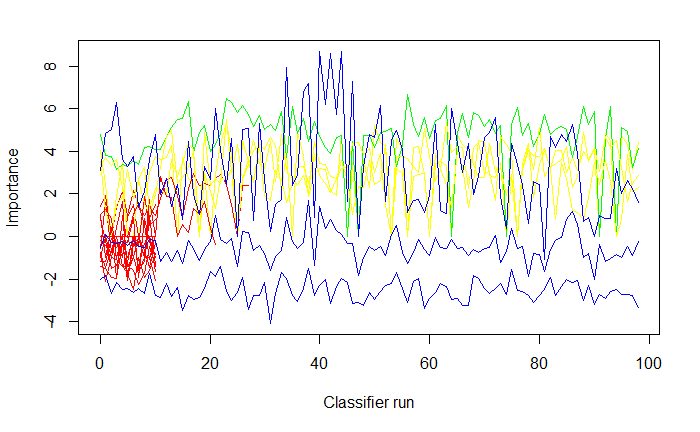
\includegraphics[scale=0.8]{graphic.png}
        \caption{Importance of each attribute during classifier run.}
        \label{fig:graphic}
    \end{figure}
    
    \item The output of getSelectedAttributes function in selected variable is a vector with the only feature selected. See Listing \ref{cod:selected-features}.
    
\begin{codefloat}[H]
\begin{lstlisting}[language=R, style=console]
[1] "npm"
\end{lstlisting}
\caption{Selected features by Boruta algorithm.}
\label{cod:selected-features}
\end{codefloat}

\end{enumerate}

The Boruta package provides an algorithm to perform feature selection. According to the results obtained, there is only one feature considered important to know if a \acrshort{oo} software has a bug and that is \acrfull{npm}.

\subsection{caret Package}
\label{sec:caret-package}

The \acrfull{caret} package contains functions to speed up the model training process for complex regression and classification problems. It has several methods that try to facilitate the process of building and evaluating the model, as well as \acrshort{fs} and other techniques \cite{caret}.

One thing to be aware of when using this package is that it loads the packages it depends on as needed and assumes they are installed. If a package is missing, a prompt appears to install it.

Using this package instead of the original method functions has two main advantages. It allows using a unified code to apply very different classification rules, implemented in different packages. It also is easier to implement some usual procedures in classification problems. For example, there are specific functions to split the sample into training data and test data or to adjust parameters through \acrlong{cv} \footnote{\acrfull{cv} is a technique used to evaluate the results of a statistical analysis and ensure that they are independent of the partition between training and test data.}.

The \acrshort{caret} R package provides tools to automatically report on the relevance and importance of attributes in your data and even select the most important features. A popular automatic wrapper method for feature selection provided by the caret R package is called \acrfull{rfe} \cite{fs-caret}. The functions of the package that are going to be needed to show an example of use are the following.

\textbf{rfe} function is the algorithm \acrshort{rfe}, a simple backwards selection algorithm. It implements backward selection based on the importance ranking of the predictors. The predictors are ranked and the less important ones are removed sequentially. For a basic use of the rfe function, it is necessary to know these arguments:

\begin{itemize}
    \item \textbf{x:} a matrix or data frame of predictors for model training. This object must have unique column names.
    
    \item \textbf{y:} a vector of results from the training set (dependent variable). It can be numeric or factor.
    
    \item \textbf{sizes:} a numeric vector of integers corresponding to the number of features that should be retained (independent features).
    
    \item \textbf{rfeControl:} a list of options, including fit and prediction functions. They are configured with the rfeControl function.
\end{itemize}

This function returns a list with two elements. The first (finalVariables) is a set of information about the execution of the algorithm that includes a top 5 of the chosen variables. The second (pred) is a data frame with columns for the accuracy metric and the kappa coefficient \footnote{The Kappa correlation coefficient is used when two or more observers must classify a set of objects each into one of several categories, or an object in one of several categories at different times or situations.}.

\textbf{rfeControl} function generates a control object that can be used to specify the details of the feature selection algorithms used in this package. The arguments of this function are:

\begin{itemize}
    \item \textbf{functions:} a list of functions for model fitting, prediction and variable importance. Some of the numerous functions that are included in the package are: lmFuncs (fitting linear models functions), rfFuncs (random forest functions), treebagFuncs (bootstrap aggregating) or nbFuncs (Naive Bayes functions).
    
    \item \textbf{method:} is the external resampling method. It can be bootstrapping (boot), \acrfull{cv}, \acrfull{loocv} or \acrfull{lgocv}.
\end{itemize}

This function returns a list with all the arguments configured in the input parameters of the function.

\textbf{predictors} function determines which predictors were used in the final model. The arguments of this function are:

\begin{itemize}
    \item \textbf{x:} can be a model object, a list, or terms that represents a model fit
\end{itemize}

This function returns a character string of the predictors selected by the model.

Knowing now the basic functions to understand how to make \acrshort{fs} with the caret package, an example of how it works will be shown. The code sequence to follow is shown in Listing \ref{cod:caret-use}.

\begin{codefloat}[H]
\begin{lstlisting}[language=R, style=Ccolor]
source("loadDataset.R")
data <- loadDataset("ckjm")

library(caret)

set.seed(2)

control <- rfeControl(functions=rfFuncs, method="cv")

results <- rfe(data[,1:20], as.factor(data$bug), sizes=c(1:20), rfeControl=control)

print(results)

selected <- predictors(results)
\end{lstlisting}
\caption{Example of caret package use.}
\label{cod:caret-use}
\end{codefloat}

The code follows these steps:

\begin{enumerate}
    \item First we use the function loadDataset (Listing \ref{cod:loadDataset.R}) to get the data from the ckjm dataset.
    
    \item We need to load caret package to use it.
    
    \item A fixed seed is then established. This is done because random components are used. The reason this is done is the same as for the Boruta package, so that the results don't change on each run. In this case a seed is set to the integer 2 but it is totally arbitrary as long as it is a constant integer.
    
    \item Now the control is defined using the random forest selection functions (rfFuncs) and the \acrfull{cv} method. These have been chosen because they are concepts already mentioned above and, therefore, are used to make \acrshort{fs} in other packages such as Boruta.
    
    \item At this point, we can run the \acrshort{rfe} algorithm. As input parameter of the predictors, the columns corresponding to the independent variables must be selected from the ckjm dataset. In this case they are the first 20, so it is selected from 1 to 20 in this way: data[,1:20]. The parameter of the vector with the data of the dependent variable must be of a numeric or factor type, but the bug is logical. To transform it into a factor, the bug data is accessed and converted as follows: as.factor(data\$bug). In this way, it only remains to specify a vector from 1 to 20 to correspond to the number of features and the control created before.
    
    \item After the algorithm runs, the results are displayed on the screen. These are made up of an explanation displayed by the console (Listing \ref{cod:caret-console}) and a data frame (Figure \ref{fig:caret-dataframe}).
    
\begin{codefloat}[H]
\begin{lstlisting}[language=R, style=console]
Recursive feature selection

Outer resampling method: Cross-Validated (10 fold) 

Resampling performance over subset size:


The top 5 variables (out of 6):
   npm, wmc, loc, cam, lcom
\end{lstlisting}
\caption{Console \acrshort{rfe} algorithm output.}
\label{cod:caret-console}
\end{codefloat}

    \begin{figure}[H]
        \centering
        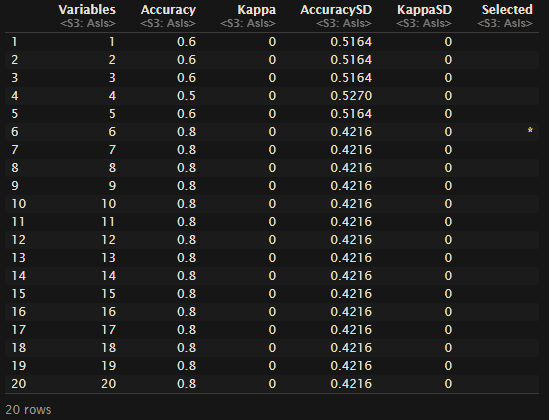
\includegraphics[scale=2]{caret-dataframe.png}
        \caption{Data frame \acrshort{rfe} algorithm output.}
        \label{fig:caret-dataframe}
    \end{figure}
    
    \item The previous step only displays a top 5 of the selected features. To know all of them, the predictors function is used with the result of the rfe algorithm as a parameter. The content of the variable selected is displayed in Listing \ref{cod:selected-caret}.
    
\begin{codefloat}[H]
\begin{lstlisting}[language=R, style=console]
[1] "npm"  "wmc"  "loc"  "cam"  "lcom" "rfc" 
\end{lstlisting}
\caption{Selected features by \acrshort{rfe} algorithm.}
\label{cod:selected-caret}
\end{codefloat}
    
\end{enumerate}

The caret package contains a large number of functions for training and plotting classification and regression models. The \acrshort{rfe} algorithm has been used to perform \acrshort{fs}. According to the results obtained, there are six features considered important to know if a \acrshort{oo} software has a bug and that are \acrfull{npm}, \acrfull{wmc}, \acrfull{loc}, \acrfull{cam}, \acrfull{lcom} and \acrfull{rfc}.

\subsection{spFSR Package}
\label{sec:spfsr-package}

The spFSR package \cite{spfsr} contains the \acrfull{spsa-fsr} algorithm as one of the wrapper methods. The \acrshort{spsa-fsr} algorithm searches for an optimal set of features that produce the best predictive performance using a specific error measure, such as the mean square error for regression problems and the accuracy rate for classification problems.

It is a package with a function with this algorithm implemented and a few functions more. It requires
an object of class task and an object of class Learner from the mlr package \cite{mlr}. To learn how to use the spFSR package, we need to know the following functions.

\textbf{spFeatureSelection} function performs \acrshort{fs} and ranking by \acrshort{spsa-fsr}. It finds the best feature subset and ranks them by their importance via the \acrfull{spsa} algorithm for a given task, wrapper, and performance criteria. The arguments of this function are:

\begin{itemize}
    \item \textbf{task:} a task object created with the mlr package. Must be ClassifTask or RegrTask object. In this case, it will be the first because it is a classification problem \footnote{Classification is the task of predicting a discrete class label.} and not a regression problem \footnote{Regression is the task of predicting a continuous quantity.}. To create a new ClassifTask object, it is used \textbf{makeClassifTask} function from mlr package with the following arguments:
    
    \begin{itemize}
        \item \textbf{data:} a data frame containing the features and target variable.
        
        \item \textbf{target:} name of the target variable.
    \end{itemize}
    
    \item \textbf{wrapper:} A Learner object created using mlr package. It has to be a classification task. To create a new Learner object, it is used \textbf{makeLearner} function from mlr package with the following argument:
    
    \begin{itemize}
        \item \textbf{cl:} class of learner. By convention, all classification learners start with “classif.”, all regression learners with “regr.”, all survival learners start with “surv.”, all clustering learners with “cluster.” and all multilabel classification learners start with “multilabel.”. The learning methods already integrated in mlr are available in \url{https://mlr.mlr-org.com/articles/tutorial/integrated_learners.html}.
    \end{itemize}
    
    \item \textbf{measure:} this is a performance measure of the mlr package which is compatible with the task. To find out which measure are compatible, you can use \textbf{listMeasures} function included in the mlr package with the following argument:
    
    \begin{itemize}
        \item \textbf{obj:} type of the task. It can be “classif”, “regr”, “surv”, “costsens”, “cluster” or “multilabel”. Default is NA matching all types.
    \end{itemize}
    
    \item \textbf{num.features.selected:} number of features to be selected. The minimum value can be 0 and the maximum the total number of functions in the task. A value of zero does not mean that no features are selected, it is that performs an automatic \acrshort{fs}.
\end{itemize}

This function returns an object of class spFSR which contains the following fields: characteristics of the defined wrapper (wrapper), measure (measure) and task (task.spfs), an mlr package WrappedModel object trained by the wrapper (best.model), a data.frame object containing detailed information on each iteration (iter.results), names of the best features (features), a vector of importance ranks of the best performing features (importance), the number of best performing features (num.features), the total number of iterations executed (total.iters), the iteration where the best performing feature subset was encountered (best.iter), the best measure value encountered (best.value), the standard deviation corresponding to the best measure value encountered (best.std), run time in minutes (run.time), resampling specification (rdesc.feat.eval) and the parameters of the function call performed (call).

\textbf{summary} function collects the most important information obtained from the results of \acrshort{fs}. The argument of this function is:

\begin{itemize}
    \item \textbf{object:} the spFSR object returned by spFeatureSelection function.
\end{itemize}

This function returns a summary of the spFSR object passed by parameter. This summary consists of target feature (target), importance of selected features (importance), number of selected features (nfeatures), number of iterations (niters), name of used wrapper (name), best iteration (best.iter), best measure value encountered (best.value), standard deviation of the best measure value (best.std) and the type of class that this function returns (attr(,"class")).

\textbf{getImportance} function extracts feature importance data from a spFSR object. The argument of this function is:

\begin{itemize}
    \item \textbf{x:} the spFSR object returned by spFeatureSelection function.
\end{itemize}

This function returns a data.frame of features and feature importance.

\textbf{plotImportance} function draw in a bar chart the importance ranks of best performing features from a spFSR object. The arguments of this function are:

\begin{itemize}
    \item \textbf{x:} the spFSR object returned by spFeatureSelection function.
    
    \item \textbf{low:} the color for the lowest importance. The default is darkblue.
    
    \item \textbf{high:} color for the highest importance. The default is black.
\end{itemize}

This function returns an image of a vertical bar chart of features versus feature importance.

As has been done with previous packages, it's time to create an example of how \acrshort{fs} works in the spFSR package. The code sequence to follow is shown in the Listing \ref{cod:spfsr-use}.

\begin{codefloat}[H]
\begin{lstlisting}[language=R, style=Ccolor]
source("loadDataset.R")
data <- loadDataset("ckjm")

library(mlr)

task <- makeClassifTask(data = data, target = "bug")

wrapper <- makeLearner("classif.knn")

listMeasures("classif")
measure <- acc

library(spFSR)
set.seed(3)

results <- spFeatureSelection(task = task, wrapper = wrapper, measure = measure, num.features.selected = 0)

summary(results)

importance <- getImportance(results)
plotImportance(results)

selected <- importance$features
\end{lstlisting}
\caption{Example of spFSR package use.}
\label{cod:spfsr-use}
\end{codefloat}

The code follows these steps:

\begin{enumerate}
    \item As before, we use the loadDataset function (Listing \ref{cod:loadDataset.R}) to get the data from the ckjm dataset.
    
    \item Next we need to load the mlr package to create the task and wrapper.
    
    \item The task is created with the makeClassifTask function setting data to the loaded dataset and target to bug.
    
    \item For the wrapper, I have chosen \acrfull{knn} \footnote{\acrlong{knn} is a supervised classification method. It is used to classify values looking for the "most similar" data points (by proximity) learned in the training stage.} to apply to the example, but it can be any classification learner that appears in the list of the previous link.
    
    \item To assign a performance measure, we query the ones available by running listMeasures function with classif parameter since we are doing a classification problem. The available measures are shown in Listing \ref{cod:available-measures}. Either one is correct and acc (accuracy) has been chosen for the example.

\begin{codefloat}[H]
\begin{lstlisting}[language=R, style=console]
 [1] "tnr"              "tpr"              "featperc"         "f1"              
 [5] "mmce"             "mcc"              "brier.scaled"     "lsr"             
 [9] "bac"              "fn"               "fp"               "fnr"             
[13] "qsr"              "fpr"              "npv"              "brier"           
[17] "auc"              "timeboth"         "multiclass.aunp"  "timetrain"       
[21] "multiclass.aunu"  "ber"              "timepredict"      "multiclass.brier"
[25] "ssr"              "ppv"              "acc"              "logloss"         
[29] "wkappa"           "tn"               "tp"               "multiclass.au1p" 
[33] "multiclass.au1u"  "fdr"              "kappa"            "gpr"             
[37] "gmean"  
\end{lstlisting}
\caption{Available measures to classification problems in mlr package.}
\label{cod:available-measures}
\end{codefloat}

    \item Now we load the spFSR package and set a seed so that the results are the same in the case of repeating the execution.
    
    \item The \acrshort{fs} is done with the spFeatureSelection function. Each input parameter is assigned the corresponding task, wrapper and measure created previously. The number of functions to select is set to 0 so that it automatically chooses the number. The output obtained during its execution is shown in Listing \ref{cod:spfsr-console}.
    
\begin{codefloat}[H]
\begin{lstlisting}[language=R, style=console]
Loading required package: parallelMap
Loading required package: parallel
Loading required package: tictoc
SPSA-FSR begins:
Wrapper = knn
Measure = acc
Number of selected features = 0

iter  value   st.dev  num.ft  best.value
1     0.6     0.33806 13      0.6 *
2     0.63333 0.35187 12      0.63333 *
3     0.6     0.33806 13      0.63333
4     0.63333 0.29681 13      0.63333
5     0.66667 0.24398 14      0.66667 *
6     0.63333 0.29681 15      0.66667
7     0.63333 0.35187 13      0.66667
8     0.63333 0.29681 13      0.66667
9     0.66667 0.30861 13      0.66667
10    0.6     0.28031 13      0.66667
11    0.63333 0.29681 11      0.66667
12    0.73333 0.2582  11      0.73333 *
13    0.63333 0.35187 11      0.73333
14    0.7     0.31623 10      0.73333
15    0.53333 0.22887 8       0.73333
16    0.73333 0.2582  9       0.73333
17    0.8     0.31623 8       0.8 *
18    0.8     0.31623 8       0.8
19    0.8     0.31623 8       0.8
20    0.8     0.25355 8       0.8
21    0.8     0.25355 8       0.8
22    0.8     0.31623 8       0.8
23    0.8     0.36839 9       0.8
24    0.8     0.31623 8       0.8
25    0.8     0.25355 8       0.8
26    0.8     0.41404 8       0.8
27    0.8     0.25355 8       0.8
28    0.8     0.25355 8       0.8
29    0.8     0.31623 8       0.8
30    0.8     0.31623 8       0.8
31    0.8     0.25355 8       0.8
32    0.8     0.31623 8       0.8
33    0.8     0.25355 8       0.8
34    0.8     0.31623 8       0.8
35    0.8     0.25355 8       0.8
36    0.8     0.31623 9       0.8
37    0.8     0.25355 9       0.8

Best iteration = 17
Number of selected features = 8
Best measure value = 0.8
Std. dev. of best measure = 0.31623
Run time = 0.27 minutes.
\end{lstlisting}
\caption{Console \acrshort{spsa-fsr} algorithm output.}
\label{cod:spfsr-console}
\end{codefloat}

    \item Listing \ref{cod:spfsr-summary} shows a summary with the most important information obtained from the result of the \acrshort{fs}.

\begin{codefloat}[H]
\begin{lstlisting}[language=R, style=console]
$target
[1] "bug"

$importance
  features importance
1      loc    0.79196
2      cbm    0.63401
3    lcom3    0.62898
4       ce    0.60143
5       ic    0.58355
6   max_cc    0.58169
7      cam    0.57527
8      amc    0.54874

$nfeatures
[1] 8

$niters
[1] 37

$name
[1] "k-Nearest Neighbor"

$best.iter
[1] 17

$best.value
[1] 0.8

$best.std
[1] 0.31623

attr(,"class")
[1] "summary.spFSR"
\end{lstlisting}
\caption{summary function output.}
\label{cod:spfsr-summary}
\end{codefloat}

    \item If we want to get a data frame with the selected features and their importance, we have the importance variable where one is stored. See Figure \ref{fig:spfsr-dataframe}. It can also be obtained in graphical form. See Figure \ref{fig:spfsr-plot}.
    
    \begin{figure}[H]
        \centering
        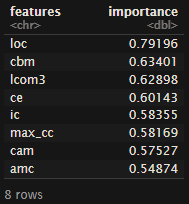
\includegraphics[scale=2.5]{spfsr-dataframe.png}
        \caption{Data frame with the selected features and their importance.}
        \label{fig:spfsr-dataframe}
    \end{figure}
    
    \begin{figure}[H]
        \centering
        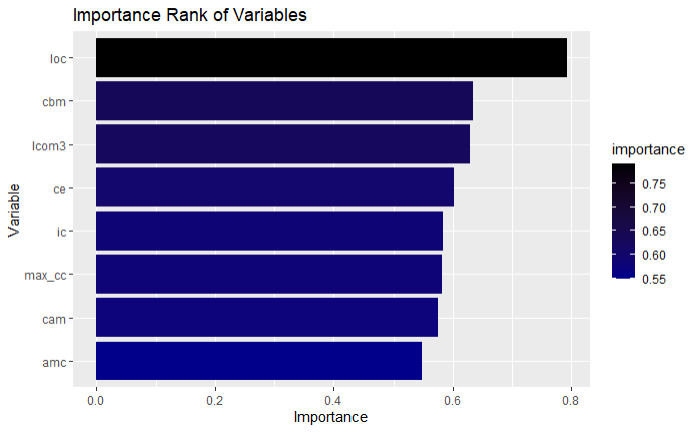
\includegraphics[scale=2.5]{spfsr-plot.png}
        \caption{Bar chart with the selected features and their importance.}
        \label{fig:spfsr-plot}
    \end{figure}
    
    \item Finally we store the names of the selected features in a vector called selected. Listing \ref{cod:spfsr-output} shows the content of this vector.

\begin{codefloat}[H]
\begin{lstlisting}[language=R, style=console]
[1] "loc"    "cbm"    "lcom3"  "ce"     "ic"     "max_cc" "cam"    "amc"  
\end{lstlisting}
\caption{Selected features by \acrshort{spsa-fsr} algorithm.}
\label{cod:spfsr-output}
\end{codefloat}

\end{enumerate}

The spFSR package only has one algorithm to perform feature selection, \acrshort{spsa-fsr}, just like the Boruta package. According to the results obtained, there are eight features considered important to know if a \acrshort{oo} software has a bug and that are \acrfull{loc}, \acrfull{cbm}, \acrfull{lcom3}, \acrfull{ce}, \acrfull{ic}, Maximum \acrlong{cc} (MAX\_\acrshort{cc}), \acrfull{cam} and \acrfull{amc}.

\subsection{varSelRF Package}
\label{sec:valselrf-package}

The valSelRF package performs random forest \acrshort{fs} using backward variable elimination, for selection of small sets of non-redundant variables, and selection based on the spectrum of importance, for selection of large and potentially highly correlated variables \cite{varselrf}.

Its main function uses the \acrfull{oob} error as minimization criterion. It consists of measuring the prediction error of random forests using bootstrap aggregation (bagging). Bagging uses subsampling with replacement to create training samples for the model to learn and evaluate predictions to immediately estimate prediction performance improvement.

To learn how to use the varSelRF package, we need to know the following functions.

varSelRF function performs \acrshort{fs} from random forests using \acrshort{oob} error as carry out variable elimination from random forest, by successively eliminating the least important variables with importance as returned from random forest. For a basic use of the varSelRF function, it is necessary to know two arguments:

\begin{itemize}
    \item \textbf{xdata:} a data frame or matrix, with observations or instances in rows and independent variables in columns.
    
    \item \textbf{Class:} the dependent variable. This argument only allows factor variable type.
    
    \item \textbf{whole.range:} if TRUE continue dropping variables until a forest with only two variables is built, and choose the best model from the complete series of models. If FALSE, stop the iterations if the current \acrshort{oob} error becomes larger than the initial or previous \acrshort{oob} error. By default it is TRUE.
\end{itemize}

This function returns an object of class varSelRF which is a list. It is made up of the following components: a data frame (selec.history) with number of variables examined (Number.Variables), variables in the forest at each stage (Vars.in.Forest), \acrlong{oob} error rate (OOB) and \acrlong{sd} of error rate (sd.OOB); the selected random forest (rf.model), the variables finally selected (selected.vars) and also ordered alphabetically (selected.model), number of variables in the finally selected model (best.model.nvars), the importances of all variables (initialImportances) and ordered in by decreasing importance (initialOrderedImportances), ntree argument (ntree) which is the number of trees to use for the first forest (by default 5000), ntreeIterat argument (ntreeIterat) which is the number of trees to use for all additional forests (by default 2000), mtryFactor argument (mtryFactor) multiplied by $\sqrt{number.of.variables}$ is used for the Random Forest input argument (by default 1) and the first forest before any variable selection fitted (firstForest).

plot function plots a varSelRF object, showing the initial variable importances, and the change in \acrshort{oob} error with the number of variables. The argument of this function is:

\begin{itemize}
    \item \textbf{x:} the varSelRF object.
\end{itemize}

This function returns two plots. The first plot is the initial importances of each variable. By default, only the 30 with the largest importance are shown but it can be changed with nvar argument. The second shows the change in \acrshort{oob} error with the number of variables.

After knowing the basic functions to understand how to do \acrshort{fs} with the varSelRF package, an example of how it works will be shown. The code sequence to follow is shown in Listing \ref{cod:varSelRF-use}.

\begin{codefloat}[H]
\begin{lstlisting}[language=R, style=Ccolor]
source("loadDataset.R")
data <- loadDataset("ckjm")

library(varSelRF)
set.seed(4)

indep <- dplyr::select(data, -bug)
dep <- as.factor(data$bug)

results <- varSelRF(indep, dep, whole.range = FALSE)

results$initialImportances[order(results$initialImportances, decreasing = T)[1:ncol(x)], 1]

plot(results)

selected <- results$selected.vars
\end{lstlisting}
\caption{Example of varSelRF package use.}
\label{cod:varSelRF-use}
\end{codefloat}

The code follows these steps:

\begin{enumerate}
    \item We use the loadDataset function (Listing \ref{cod:loadDataset.R}) to get the data from the ckjm dataset.
    
    \item Now we load the spFSR package to use it and set a seed so that the results are the same in the case of repeating the execution.
    
    \item We separate the data corresponding to the independent variables from the data of the dependent variable. The select function found inside the dplyr package is used to get the independent variables. From all the data (data) the dependent variable (-bug) is removed. To obtain only the dependent variable, only the bug column of the data is taken. Since the input argument of the varSelRF function has to be of type factor, the conversion from logical to factor is done with as.factor.
    
    \item The necessary arguments of the varSelRF function are filled in to perform the \acrshort{fs}. The first is the independent variables, the second is the dependent variable, both selected above. The third is whole.range set to FALSE so that it stops iterating if the current \acrshort{oob} error becomes larger than the initial or previous \acrshort{oob} error.
    
    \item To visualize the calculated importance, the initialImportances component of the results obtained from the \acrshort{fs} is consulted. It is ordered from smallest to largest and the names of the variables that correspond to each of the importance are added. See Listing \ref{cod:varselrf-importance}. This is done for a better understanding of the graph of Figure \ref{fig:varselrf-plot1}.
    
\begin{codefloat}[H]
\begin{lstlisting}[language=R, style=console]
       avg_cc         lcom3           moa            ca           mfa 
-0.0058133333 -0.0035100000 -0.0034733333 -0.0033666667 -0.0020600000 
       max_cc           dit           cbo            ce           dam 
-0.0019833333 -0.0015000000 -0.0011466667 -0.0010071429 -0.0003466667 
          noc            ic           cbm           rfc           amc 
 0.0000000000  0.0000000000  0.0000000000  0.0011833333  0.0031528571 
         lcom           cam           loc           wmc           npm 
 0.0064333333  0.0178366667  0.0197666667  0.0245233333  0.0332238095 
\end{lstlisting}
\caption{Importance of independent features.}
\label{cod:varselrf-importance}
\end{codefloat}

    \item The plot of Figure \ref{fig:varselrf-plot1} is the initial importances of each variable. Since there are 20 variables, it does not affect the restriction that only the 30 largest are displayed. The plot of Figure \ref{fig:varselrf-plot2} shows the change in \acrshort{oob} error with the number of variables.
    
    \begin{figure}[H]
        \centering
        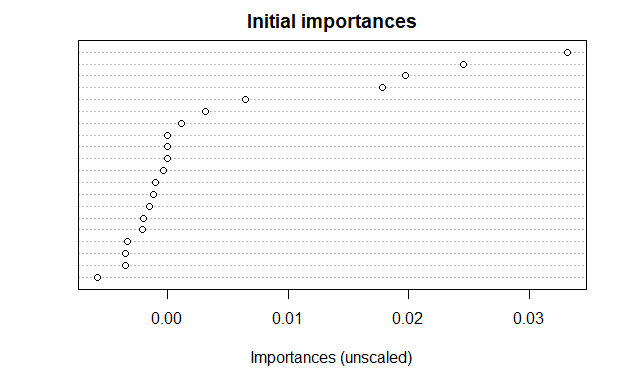
\includegraphics[scale=0.9]{varselrf-plot1.png}
        \caption{Plot of the initial importances of each variable.}
        \label{fig:varselrf-plot1}
    \end{figure}
    
    \begin{figure}[H]
        \centering
        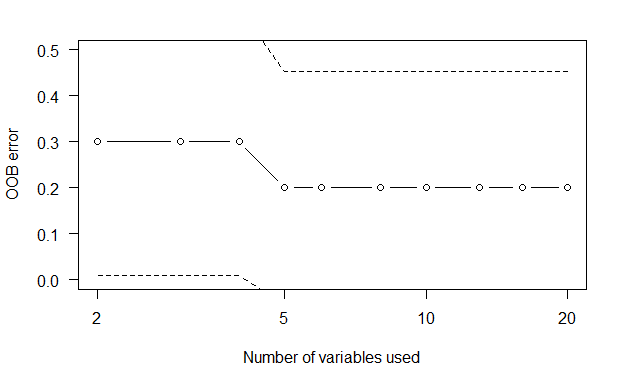
\includegraphics[scale=0.9]{varselrf-plot2.png}
        \caption{Plot of the change in \acrshort{oob} error with the number of variables.}
        \label{fig:varselrf-plot2}
    \end{figure}
    
    \item Finally we store the names of the selected features in a vector called selected. Listing \ref{cod:varselrf-output} shows the content of this vector.

\begin{codefloat}[H]
\begin{lstlisting}[language=R, style=console]
[1] "npm" "wmc"
\end{lstlisting}
\caption{Selected features by varSelRF function.}
\label{cod:varselrf-output}
\end{codefloat}

\end{enumerate}

The varSelRF package only has one algorithm to perform feature selection, backward variable elimination with \acrshort{oob} error as minimization criterion, just like the spFSR or Boruta package. According to the results obtained, there are two features considered important to know if a \acrshort{oo} software has a bug and that are \acrfull{npm} and \acrfull{wmc}.

\subsection{Other important packages}
\label{sec:other-packages}

Other useful packages for information on data and feature selection will be introduced in this section. These packages are not used to perform the selection of features but they help to obtain very useful metrics to study and better understand the process.

\subsubsection{SHAPforxgboost Package}
\label{sec:shap-package}

The R package SHAPforxgboost computes SHAP values using an XGBoost (Extreme Gradient Boosting) classifier, very popular in kaggle.com competitions \footnote{\url{https://www.kaggle.com/competitions}}.

The xalan-2.7 dataset will be used since of the chosen datasets it is the one that contains the most modules. This will be a benefit for better visualization.

The classification problem consists of knowing if a \acrshort{oo} software contains a module with a bug (TRUE) or not (FALSE), based on some predictor-parameters of the \acrshort{ck} metric. What we are interested in are the SHAP-values of these for each metric.

We need \textbf{xgboost} function from xgboost package to train the model. The main arguments of this function are:

\begin{itemize}
    \item \textbf{data:} training dataset. It is a matrix with independent variables of dataset.
    
    \item \textbf{label:} vector of response values (dependent variable).
    
    \item \textbf{nrounds:} max number of boosting iterations.
\end{itemize}

This function returns an object of class xgb.Booster.

The functions of the SHAPforxgboost package that we need to know about are the following.

\textbf{shap.values} function gets SHAP scores from a trained XGBoost model. The arguments of this function are:

\begin{itemize}
    \item \textbf{xgb\_model:} an XGBoost model object.

    \item \textbf{X\_train:} the dataset of predictors (independent variables) used for calculating SHAP values, it should be a matrix.
\end{itemize}

This function returns a list of three objects from XGBoost model: a dataset of SHAP scores, the ranked variable vector by each variable’s mean absolute SHAP value and the BIAS, which is like an intercept.

\textbf{shap.prep} function prepares SHAP values into long format for plotting. The main arguments of this function are:

\begin{itemize}
    \item \textbf{xgb\_model:} an XGBoost model object, will derive the SHAP values from it.

    \item \textbf{X\_train:} the dataset of predictors used to calculate SHAP values, it provides feature values to the plot, must be supplied.
\end{itemize}

This function returns a dataset of 6 columns: ID of each observation, variable name, SHAP value, variable values
(feature value), deviation of the feature value for each observation (for coloring the point), and the
mean SHAP values for each variable.

\textbf{shap.plot.summary} function uses the long format SHAP values to create the SHAP summary plot. The argument os this function is:

\begin{itemize}
    \item \textbf{data\_long:} a long format data of SHAP values from shap.prep function.
\end{itemize}

This function returns a plot with the SHAP values of each feature.

Now we are going to test how the SHAP values are calculated with the code of the Listing \ref{cod:shap-use}.

\begin{codefloat}[H]
\begin{lstlisting}[language=R, style=Ccolor]
source("./loadDataset.R")
data <- loadDataset("xalan-2.7")

library("SHAPforxgboost")
X = as.matrix(dplyr::select(data, -bug))

mod = xgboost::xgboost(data = X, label = data$bug, nrounds = 1)

shap_values <- shap.values(xgb_model = mod, X_train = X)
shap_values$mean_shap_score

shap_long_data <- shap.prep(xgb_model = mod, X_train = X)

shap.plot.summary(shap_long_data)
\end{lstlisting}
\caption{Example of SHAP values with SHAPforxgboost package.}
\label{cod:shap-use}
\end{codefloat}

The code follows these steps:

\begin{enumerate}
    \item First, we load xalan-2.7 dataset with loadDataset function (Listing \ref{cod:loadDataset.R}).
    
    \item The next step is to load the SHAPforxgboost package and select from the dataset only the independent variables. It is then converted to a matrix and stored in a variable (X) so that it can be passed as a parameter to the following functions.
    
    \item Now the model is trained with the xgboost function from the package with the same name. X variable is data paremeter, the label is the bug data and nrounds is set to 1 (no more is needed for this example).
    
    \item SHAP values are calculated with the parameters xgb\_model as the result of previous function and Xtrain as X variable. Then we can see the mean of SHAP values with \$mean\_shap\_score in Listing \ref{cod:shap-output}.
    
\begin{codefloat}[H]
\begin{lstlisting}[language=R, style=console]
         npm          cam         lcom        lcom3          wmc          dit 
0.0072010987 0.0047268687 0.0021199110 0.0014011440 0.0004532199 0.0002328541 
         noc          cbo          rfc           ca           ce          loc 
0.0000000000 0.0000000000 0.0000000000 0.0000000000 0.0000000000 0.0000000000 
         dam          moa          mfa           ic          cbm          amc 
0.0000000000 0.0000000000 0.0000000000 0.0000000000 0.0000000000 0.0000000000 
      max_cc       avg_cc 
0.0000000000 0.0000000000 
\end{lstlisting}
\caption{Mean of the SHAP values of the variables.}
\label{cod:shap-output}
\end{codefloat}

    \item The results are prepared for display using the shap.prep function with the same parameters as the previous function.
    
    \item Finally the SHAP values are plotted. Figure \ref{fig:shap-values-plot}.
        \begin{figure}[H]
            \centering
            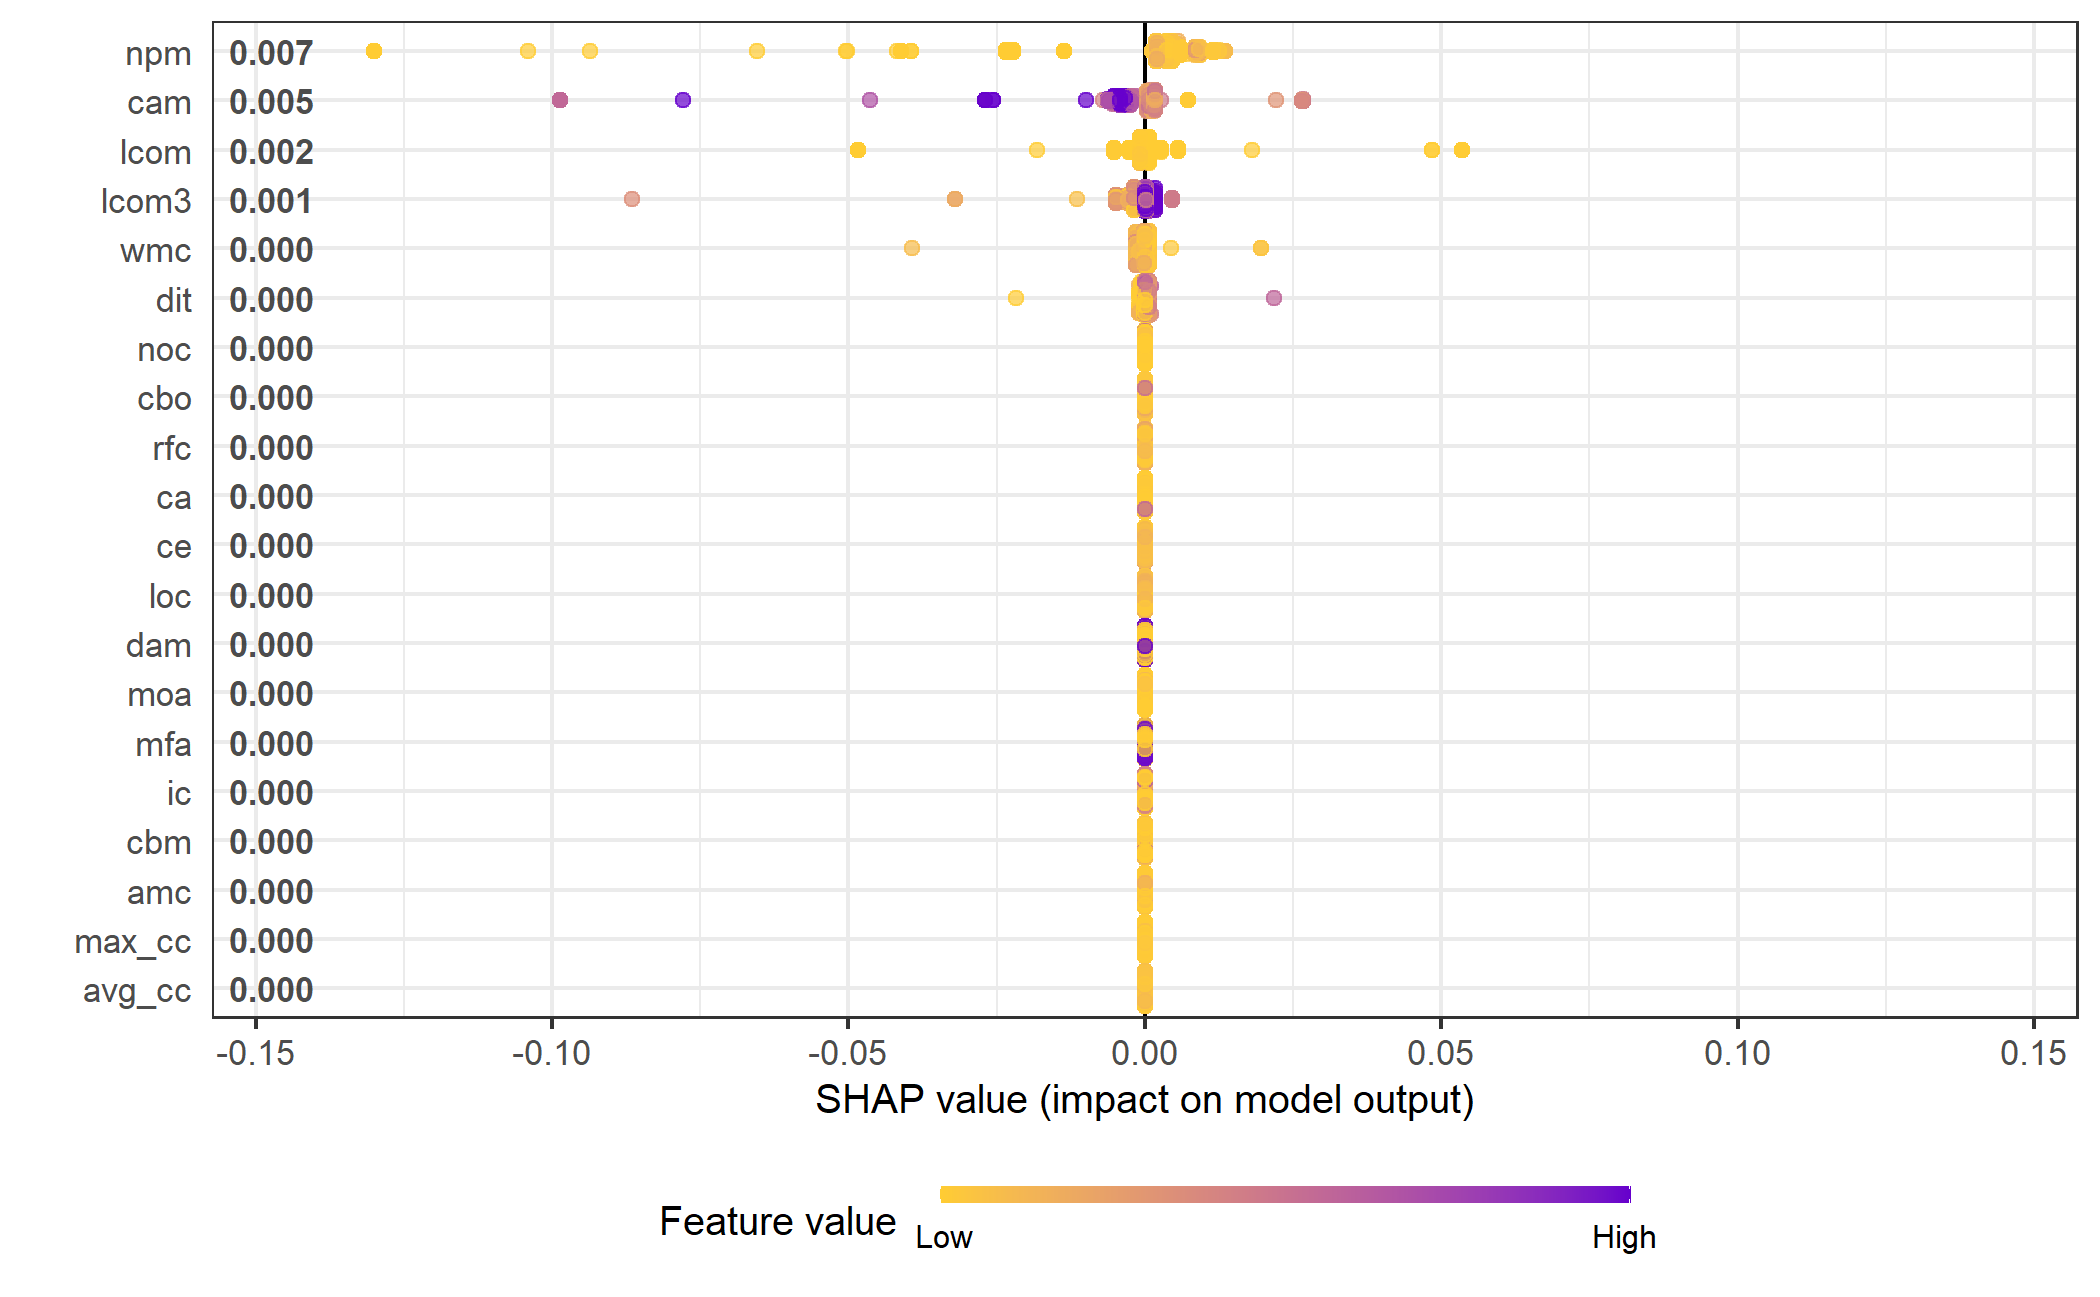
\includegraphics[scale=0.8]{shap-values.png}
            \caption{SHAP values plot.}
            \label{fig:shap-values-plot}
        \end{figure}
    
    Figure \ref{fig:shap-values-plot} shows, in point cloud format, the SHAP values for each value of each variable. Each point comes to represent a case, with its corresponding value in each independent variable: variables, on the left vertical axis, aligned. The value of SHAP, on the horizontal axis. The low values of the variables are shown in yellow and the high values in purple (it can be seen on the horizontal axis at the bottom). For example, in the variable \acrshort{cam} you can see how high values (purple) tend to have a negative result (left of the vertical separation), that is, with a higher value of \acrshort{cam}, the bug variable tends to be false.
\end{enumerate}

\subsubsection{ECol Package}
\label{sec:ecol-package}

The R package \acrfull{ecol} contains different complexity measures for supervised problems as \acrlong{fs}. It provides measures to characterize the complexity of classification and regression problems based on aspects that quantify the linearity of the data, the presence of informative feature, the sparsity and dimensionality of the datasets \cite{ecol-article}.

The measures can be divided into two groups: classification and regression measures. The classification measures are based on: feature-based measures, neighborhood measures, linearity measures, dimensionality measures, class balance measures and network measures. The regression measures are based on: linearity measures, dimensionality measures, correlation measures and smoothness measures.

\textbf{Feature-based measures}

\begin{itemize}
    \item F1: Fisher's discriminant ratio.
    \item F1v: The directional-vector Fisher's discriminant ratio.
    \item F2: Overlapping of the per-class bounding boxes.
    \item F3: Maximum individual feature efficiency.
    \item F4: Collective feature efficiency.
\end{itemize}
    
\textbf{Neighborhood information}

\begin{itemize}
    \item N1: Fraction of points lying on the class boundary.
    \item N2: Average intra/inter class nearest neighbor distances.
    \item N3: Leave-one-out error rate of the 1-nearest neighbor algorithm.
    \item N4: Nonlinearity of the one-nearest neighbor classifier.
    \item N5: Fraction of maximum covering spheres on data.
    \item N6: Local-Set cardinality average.
\end{itemize}

\textbf{Linearity}

\begin{itemize}
    \item L1: Distance of erroneous instances to a linear classifier.
    \item L2: Training error of a linear classifier.
    \item L3: Nonlinearity of a linear classifier.
\end{itemize}

\textbf{Dimensionality}

\begin{itemize}
    \item D1: Average number of samples per dimension.
    \item D2: Average intrinsic dimensionality per number of examples.
    \item D3: Intrinsic dimensionality proportion.
\end{itemize}

\textbf{Class balance}

\begin{itemize}
    \item B1: Entropy of class proportions.
    \item B2: Multi-class imbalance ratio.
\end{itemize}

\textbf{Structural representation}

\begin{itemize}
    \item G1: Average density of network.
    \item G2: Clustering Coefficient.
    \item G3: Average hub score.
\end{itemize}

\textbf{Feature correlation}

\begin{itemize}
    \item C1: Feature correlation to the output.
    \item C2: Average feature correlation to the output.
    \item C3: Individual feature efficiency.
    \item C4: Collective feature efficiency.
\end{itemize}

\textbf{Smoothness}

\begin{itemize}
    \item S1: Output distribution.
    \item S2: Input distribution.
    \item S3: Error of a nearest neighbor regressor.
    \item S4: Non-linearity of nearest neighbor regressor.
\end{itemize}

\textbf{complexity} function is the main function of \acrshort{ecol} package. It is responsable to extract the complexity measures from the classification and regression tasks. The simplest way to compute the complexity measures are using this function. The function can be called by a symbolic description of the model or by a data frame. If it is a classification task, the output varriable needs to be a factor, otherwise the package will assume a regression task. The arguments to be used for this function are:

\begin{itemize}
    \item \textbf{formula:} A formula to define the output column.
    \item \textbf{data:} A data.frame dataset contained the input and output attributes.
    \item \textbf{summary:} A list of summarization functions or empty for all values. By default they are media and \acrshort{sd}.
\end{itemize}

This function returns a numeric vector named by the requested complexity measures. The default parameter is extract all the measures. To extract a specific measure, use the function related with the group. Available functions are balance, correlation, dimensionality, linearity, neighborhood, network, overlapping and smoothness.

To calculate the complexity, the code in Listing \ref{cod:complexity-use} is executed.

\begin{codefloat}[H]
\begin{lstlisting}[language=R, style=Ccolor]
complexity(as.factor(bug) ~ ., data)
\end{lstlisting}
\caption{Example of use of the function complexity.}
\label{cod:complexity-use}
\end{codefloat}

In Section \ref{sec:complexity-fsinr} the complexity in the FSinR package will be calculated.

\section{Measures in FSinR package}
\label{sec:measures-fsinr}

In this section, the function applyFSinR (Listing \ref{cod:applyFSinR.R}) is used to select attributes by applying all the search algorithms contained in the FSinR package to each of the datasets chosen in Section \ref{sec:fsinr-package}. Then the complexity and stability of the results obtained in the following sections (Section \ref{sec:complexity-fsinr} and Section \ref{sec:stability-fsinr} respectively) will be calculated.

The function to use to apply the applyFSinR function to the different datasets is \textbf{mapply}. The arguments of this function are:

\begin{itemize}
    \item \textbf{FUN:} function to apply.
    \item \textbf{args:} input arguments for the function parameter FUN. It must be a list or a vector.
    \item \textbf{MoreArgs:} a list of other arguments to FUN.
\end{itemize}

It returns a list where first element is the result of applies FUN to the first elements of each argument, the second element is the result of second elements, and so on.

Since the applyFSinR function returns a list, applying mapply to it will create a matrix. The different datasets will appear in the columns of this matrix and the features will appear in the rows. The features marked with 1 means that it has been selected and 0 that it has not.

Remember that the search algorithms of the FSinR packages are:
\begin{itemize}
    \item sequentialForwardSelection: \acrfull{sfs}.
    \item sequentialFloatingForwardSelection: \acrfull{sffs}
    \item sequentialBackwardSelection: \acrfull{sbs}
    \item sequentialFloatingBackwardSelection: \acrfull{sfbs}
    \item breadthFirst: Breadth first search
    \item deepFirst: Deep first search
    \item geneticAlgorithm: \acrfull{ga}
    \item whaleOptimization: \acrfull{woa}
    \item antColony: \acrfull{aco}
    \item simulatedAnnealing: \acrfull{sa}
    \item tabu: \acrfull{ts}
    \item hillClimbing: \acrfull{hc}
    \item LasVegas: \acrfull{lv}
\end{itemize}

How to use the mapply function with these algorithms is shown in Listing \ref{cod:mapply-use}.

\begin{codefloat}[H]
\begin{lstlisting}[language=R, style=Ccolor]
source("./loadDataset.R")
source("./applyFSinR.R")

FSMatrix <- mapply(applyFSinR, dsnames, algorithm='sequentialForwardSelection')
\end{lstlisting}
\caption{Example of use of the function mapply with search algorithms.}
\label{cod:mapply-use}
\end{codefloat}

The code follows these steps:

\begin{enumerate}
    \item Load loadDataset.R (Listing \ref{cod:loadDataset.R}) and applyFSinR.R.
    
    \item Use mapply with the applyFSinR function and the dataset names (dsnames) as a parameter.
    
    \item Set the algorithm to use for \acrshort{fs} of all datasets.
\end{enumerate}

The output results of the \acrshort{fs} made with each of the algorithms are shown in the following tables (Appendix \ref{cha:fsinr-fs}):

\begin{itemize}
    \item Table \ref{tab:sfs-output}: \acrlong{sfs}.
    \item Table \ref{tab:sffs-output}: \acrlong{sffs}.
    \item Table \ref{tab:sbs-output}: \acrlong{sbs}.
    \item Table \ref{tab:sfbs-output}: \acrlong{sfbs}.
    \item Breadth first search: Its execution takes a long time. No output has been achieved.
    \item Deep first search: Its execution takes a long time. No output has been achieved.
    \item \acrlong{ga}: Returns a data frame with several results. It is discarded for not respecting the format.
    \item Table \ref{tab:woa-output}: \acrlong{woa}.
    \item \acrlong{aco}: Returns a repetitive unresolved warning. No output has been achieved.
    \item \acrlong{sa}: Returns a data frame with several results. It is discarded for not respecting the format.
    \item Table \ref{tab:ts-output}: \acrlong{ts}.
    \item Table \ref{tab:hc-output}: \acrlong{hc}.
    \item Table \ref{tab:lv-output}: \acrlong{lv}.
\end{itemize}

With the results obtained and the format adopted, it is much easier to calculate the complexity and stability of the \acrshort{fs} in the following sections.

\subsection{Complexity in FSinR package}
\label{sec:complexity-fsinr}

As previous examples, the ckjm dataset will be used to demonstrate the use of the \acrshort{ecol} package to calculate complexity. First the complexity of the dataset will be calculated without performing the \acrshort{fs}. Then it will be calculated on the selection made to the ckjm dataset with the different search algorithms that have been executed from the FSinR package.

With the code of Listing \ref{cod:complexity-use} we can calculate the complexity by changing the data variable for what corresponds to each execution.

The results obtained are the following:

\begin{itemize}
    \item Listing \ref{cod:complexity-initial}: Without \acrshort{fs}.
    
\begin{codefloat}[H]
\begin{lstlisting}[language=R, style=console]
 overlapping.F1.mean    overlapping.F1.sd overlapping.F1v.mean   overlapping.F1v.sd  overlapping.F2.mean 
          0.87431831           0.11405331           0.02400049                   NA           0.00000000 
   overlapping.F2.sd  overlapping.F3.mean    overlapping.F3.sd  overlapping.F4.mean    overlapping.F4.sd 
                  NA           0.40000000                   NA           0.00000000                   NA 
     neighborhood.N1 neighborhood.N2.mean   neighborhood.N2.sd neighborhood.N3.mean   neighborhood.N3.sd 
          0.70000000           0.54015910           0.11935810           0.50000000           0.52704628 
neighborhood.N4.mean   neighborhood.N4.sd neighborhood.T1.mean   neighborhood.T1.sd     neighborhood.LSC 
          0.00000000           0.00000000           0.12500000           0.04629100           0.84000000 
   linearity.L1.mean      linearity.L1.sd    linearity.L2.mean      linearity.L2.sd    linearity.L3.mean 
          0.00000000                   NA           0.00000000                   NA           0.00000000 
     linearity.L3.sd    dimensionality.T2    dimensionality.T3    dimensionality.T4           balance.C1 
                  NA           2.00000000           0.20000000           0.10000000           1.00000000 
          balance.C2      network.Density      network.ClsCoef    network.Hubs.mean      network.Hubs.sd 
          0.00000000           0.91111111           1.00000000           0.80000000           0.42163702 
\end{lstlisting}
\caption{Complexity measures of dataset without \acrshort{fs}.}
\label{cod:complexity-initial}
\end{codefloat}

    \item Listing \ref{cod:complexity-sfs}: \acrshort{fs} with \acrlong{sfs}.
    
\begin{codefloat}[H]
\begin{lstlisting}[language=R, style=console]
 overlapping.F1.mean    overlapping.F1.sd overlapping.F1v.mean   overlapping.F1v.sd  overlapping.F2.mean 
         0.847089728          0.143618400          0.010557789                   NA          0.001122329 
   overlapping.F2.sd  overlapping.F3.mean    overlapping.F3.sd  overlapping.F4.mean    overlapping.F4.sd 
                  NA          0.400000000                   NA          0.000000000                   NA 
     neighborhood.N1 neighborhood.N2.mean   neighborhood.N2.sd neighborhood.N3.mean   neighborhood.N3.sd 
         0.600000000          0.496209376          0.080669720          0.400000000          0.516397779 
neighborhood.N4.mean   neighborhood.N4.sd neighborhood.T1.mean   neighborhood.T1.sd     neighborhood.LSC 
         0.000000000          0.000000000          0.125000000          0.046291005          0.800000000 
   linearity.L1.mean      linearity.L1.sd    linearity.L2.mean      linearity.L2.sd    linearity.L3.mean 
         0.000000000                   NA          0.000000000                   NA          0.000000000 
     linearity.L3.sd    dimensionality.T2    dimensionality.T3    dimensionality.T4           balance.C1 
                  NA          0.900000000          0.100000000          0.111111111          1.000000000 
          balance.C2      network.Density      network.ClsCoef    network.Hubs.mean      network.Hubs.sd 
         0.000000000          0.888888889          1.000000000          0.752072976          0.377648116 
\end{lstlisting}
\caption{Complexity measures of dataset with \acrshort{sfs}.}
\label{cod:complexity-sfs}
\end{codefloat}

    \item Listing \ref{cod:complexity-sffs}: \acrshort{fs} with \acrlong{sffs}.
    
\begin{codefloat}[H]
\begin{lstlisting}[language=R, style=console]
 overlapping.F1.mean    overlapping.F1.sd overlapping.F1v.mean   overlapping.F1v.sd  overlapping.F2.mean 
         0.847089728          0.143618400          0.010557789                   NA          0.001122329 
   overlapping.F2.sd  overlapping.F3.mean    overlapping.F3.sd  overlapping.F4.mean    overlapping.F4.sd 
                  NA          0.400000000                   NA          0.000000000                   NA 
     neighborhood.N1 neighborhood.N2.mean   neighborhood.N2.sd neighborhood.N3.mean   neighborhood.N3.sd 
         0.600000000          0.496209376          0.080669720          0.400000000          0.516397779 
neighborhood.N4.mean   neighborhood.N4.sd neighborhood.T1.mean   neighborhood.T1.sd     neighborhood.LSC 
         0.000000000          0.000000000          0.125000000          0.046291005          0.800000000 
   linearity.L1.mean      linearity.L1.sd    linearity.L2.mean      linearity.L2.sd    linearity.L3.mean 
         0.000000000                   NA          0.000000000                   NA          0.000000000 
     linearity.L3.sd    dimensionality.T2    dimensionality.T3    dimensionality.T4           balance.C1 
                  NA          0.900000000          0.100000000          0.111111111          1.000000000 
          balance.C2      network.Density      network.ClsCoef    network.Hubs.mean      network.Hubs.sd 
         0.000000000          0.888888889          1.000000000          0.752072976          0.377648116 
\end{lstlisting}
\caption{Complexity measures of dataset with \acrshort{sffs}.}
\label{cod:complexity-sffs}
\end{codefloat}

    \item Listing \ref{cod:complexity-sbs}: \acrshort{fs} with \acrlong{sbs}.
    
\begin{codefloat}[H]
\begin{lstlisting}[language=R, style=console]
 overlapping.F1.mean    overlapping.F1.sd overlapping.F1v.mean   overlapping.F1v.sd  overlapping.F2.mean 
          0.86512689           0.12475894           0.02374944                   NA           0.00000000 
   overlapping.F2.sd  overlapping.F3.mean    overlapping.F3.sd  overlapping.F4.mean    overlapping.F4.sd 
                  NA           0.40000000                   NA           0.00000000                   NA 
     neighborhood.N1 neighborhood.N2.mean   neighborhood.N2.sd neighborhood.N3.mean   neighborhood.N3.sd 
          0.70000000           0.51674109           0.13843808           0.50000000           0.52704628 
neighborhood.N4.mean   neighborhood.N4.sd neighborhood.T1.mean   neighborhood.T1.sd     neighborhood.LSC 
          0.00000000           0.00000000           0.14285714           0.05345225           0.85000000 
   linearity.L1.mean      linearity.L1.sd    linearity.L2.mean      linearity.L2.sd    linearity.L3.mean 
          0.00000000                   NA           0.00000000                   NA           0.00000000 
     linearity.L3.sd    dimensionality.T2    dimensionality.T3    dimensionality.T4           balance.C1 
                  NA           0.90000000           0.10000000           0.11111111           1.00000000 
          balance.C2      network.Density      network.ClsCoef    network.Hubs.mean      network.Hubs.sd 
          0.00000000           0.91111111           1.00000000           0.80000000           0.42163702 
\end{lstlisting}
\caption{Complexity measures of dataset with \acrshort{sbs}.}
\label{cod:complexity-sbs}
\end{codefloat}

    \item Listing \ref{cod:complexity-sfbs}: \acrshort{fs} with \acrlong{sfbs}.
    
\begin{codefloat}[H]
\begin{lstlisting}[language=R, style=console]
 overlapping.F1.mean    overlapping.F1.sd overlapping.F1v.mean   overlapping.F1v.sd  overlapping.F2.mean 
          0.86512689           0.12475894           0.02374944                   NA           0.00000000 
   overlapping.F2.sd  overlapping.F3.mean    overlapping.F3.sd  overlapping.F4.mean    overlapping.F4.sd 
                  NA           0.40000000                   NA           0.00000000                   NA 
     neighborhood.N1 neighborhood.N2.mean   neighborhood.N2.sd neighborhood.N3.mean   neighborhood.N3.sd 
          0.70000000           0.51674109           0.13843808           0.50000000           0.52704628 
neighborhood.N4.mean   neighborhood.N4.sd neighborhood.T1.mean   neighborhood.T1.sd     neighborhood.LSC 
          0.10000000           0.31622777           0.14285714           0.05345225           0.85000000 
   linearity.L1.mean      linearity.L1.sd    linearity.L2.mean      linearity.L2.sd    linearity.L3.mean 
          0.00000000                   NA           0.00000000                   NA           0.00000000 
     linearity.L3.sd    dimensionality.T2    dimensionality.T3    dimensionality.T4           balance.C1 
                  NA           0.90000000           0.10000000           0.11111111           1.00000000 
          balance.C2      network.Density      network.ClsCoef    network.Hubs.mean      network.Hubs.sd 
          0.00000000           0.91111111           1.00000000           0.80000000           0.42163702 
\end{lstlisting}
\caption{Complexity measures of dataset with \acrshort{sfbs}.}
\label{cod:complexity-sfbs}
\end{codefloat}

    \item Listing \ref{cod:complexity-woa}: \acrshort{fs} with \acrlong{woa}.
    
\begin{codefloat}[H]
\begin{lstlisting}[language=R, style=console]
 overlapping.F1.mean    overlapping.F1.sd overlapping.F1v.mean   overlapping.F1v.sd  overlapping.F2.mean 
         0.804209143          0.117538998          0.007866884                   NA          0.000000000 
   overlapping.F2.sd  overlapping.F3.mean    overlapping.F3.sd  overlapping.F4.mean    overlapping.F4.sd 
                  NA          0.400000000                   NA          0.000000000                   NA 
     neighborhood.N1 neighborhood.N2.mean   neighborhood.N2.sd neighborhood.N3.mean   neighborhood.N3.sd 
         0.600000000          0.489863067          0.117760757          0.400000000          0.516397779 
neighborhood.N4.mean   neighborhood.N4.sd neighborhood.T1.mean   neighborhood.T1.sd     neighborhood.LSC 
         0.000000000          0.000000000          0.142857143          0.078679579          0.800000000 
   linearity.L1.mean      linearity.L1.sd    linearity.L2.mean      linearity.L2.sd    linearity.L3.mean 
         0.050018870                   NA          0.100000000                   NA          0.000000000 
     linearity.L3.sd    dimensionality.T2    dimensionality.T3    dimensionality.T4           balance.C1 
                  NA          0.900000000          0.100000000          0.111111111          1.000000000 
          balance.C2      network.Density      network.ClsCoef    network.Hubs.mean      network.Hubs.sd 
         0.000000000          0.888888889          1.000000000          0.812419332          0.347377200 
\end{lstlisting}
\caption{Complexity measures of dataset with \acrshort{woa}.}
\label{cod:complexity-woa}
\end{codefloat}

    \item Listing \ref{cod:complexity-ts}: \acrshort{fs} with \acrlong{ts}.
    
\begin{codefloat}[H]
\begin{lstlisting}[language=R, style=console]
 overlapping.F1.mean    overlapping.F1.sd overlapping.F1v.mean   overlapping.F1v.sd  overlapping.F2.mean 
        0.8538614897         0.0970090467         0.0830652473                   NA         0.0002991075 
   overlapping.F2.sd  overlapping.F3.mean    overlapping.F3.sd  overlapping.F4.mean    overlapping.F4.sd 
                  NA         0.4000000000                   NA         0.0000000000                   NA 
     neighborhood.N1 neighborhood.N2.mean   neighborhood.N2.sd neighborhood.N3.mean   neighborhood.N3.sd 
        0.7000000000         0.5317091201         0.1291913579         0.5000000000         0.5270462767 
neighborhood.N4.mean   neighborhood.N4.sd neighborhood.T1.mean   neighborhood.T1.sd     neighborhood.LSC 
        0.0000000000         0.0000000000         0.1250000000         0.0462910050         0.8500000000 
   linearity.L1.mean      linearity.L1.sd    linearity.L2.mean      linearity.L2.sd    linearity.L3.mean 
        0.0380116930                   NA         0.1000000000                   NA         0.1000000000 
     linearity.L3.sd    dimensionality.T2    dimensionality.T3    dimensionality.T4           balance.C1 
                  NA         0.9000000000         0.3000000000         0.3333333333         1.0000000000 
          balance.C2      network.Density      network.ClsCoef    network.Hubs.mean      network.Hubs.sd 
        0.0000000000         0.9111111111         1.0000000000         0.8000000000         0.4216370214 
\end{lstlisting}
\caption{Complexity measures of dataset with \acrshort{ts}.}
\label{cod:complexity-ts}
\end{codefloat}

    \item Listing \ref{cod:complexity-hc}: \acrshort{fs} with \acrlong{hc}.
    
\begin{codefloat}[H]
\begin{lstlisting}[language=R, style=console]
 overlapping.F1.mean    overlapping.F1.sd overlapping.F1v.mean   overlapping.F1v.sd  overlapping.F2.mean 
          0.91079687           0.10431029           0.02428087                   NA           0.00000000 
   overlapping.F2.sd  overlapping.F3.mean    overlapping.F3.sd  overlapping.F4.mean    overlapping.F4.sd 
                  NA           0.40000000                   NA           0.00000000                   NA 
     neighborhood.N1 neighborhood.N2.mean   neighborhood.N2.sd neighborhood.N3.mean   neighborhood.N3.sd 
          0.70000000           0.57006599           0.17855876           0.50000000           0.52704628 
neighborhood.N4.mean   neighborhood.N4.sd neighborhood.T1.mean   neighborhood.T1.sd     neighborhood.LSC 
          0.10000000           0.31622777           0.12500000           0.04629100           0.83000000 
   linearity.L1.mean      linearity.L1.sd    linearity.L2.mean      linearity.L2.sd    linearity.L3.mean 
          0.08161969                   NA           0.10000000                   NA           0.10000000 
     linearity.L3.sd    dimensionality.T2    dimensionality.T3    dimensionality.T4           balance.C1 
                  NA           0.90000000           0.30000000           0.33333333           1.00000000 
          balance.C2      network.Density      network.ClsCoef    network.Hubs.mean      network.Hubs.sd 
          0.00000000           0.91111111           1.00000000           0.80000000           0.42163702 
\end{lstlisting}
\caption{Complexity measures of dataset with \acrshort{hc}.}
\label{cod:complexity-hc}
\end{codefloat}

    \item Listing \ref{cod:complexity-lv}: \acrshort{fs} with \acrlong{lv}.
    
\begin{codefloat}[H]
\begin{lstlisting}[language=R, style=console]
 overlapping.F1.mean    overlapping.F1.sd overlapping.F1v.mean   overlapping.F1v.sd  overlapping.F2.mean 
          0.91039918           0.10492237           0.03929172                   NA           0.00000000 
   overlapping.F2.sd  overlapping.F3.mean    overlapping.F3.sd  overlapping.F4.mean    overlapping.F4.sd 
                  NA           0.40000000                   NA           0.00000000                   NA 
     neighborhood.N1 neighborhood.N2.mean   neighborhood.N2.sd neighborhood.N3.mean   neighborhood.N3.sd 
          0.70000000           0.55675532           0.13836897           0.60000000           0.51639778 
neighborhood.N4.mean   neighborhood.N4.sd neighborhood.T1.mean   neighborhood.T1.sd     neighborhood.LSC 
          0.10000000           0.31622777           0.12500000           0.04629100           0.86000000 
   linearity.L1.mean      linearity.L1.sd    linearity.L2.mean      linearity.L2.sd    linearity.L3.mean 
          0.10850133                   NA           0.10000000                   NA           0.10000000 
     linearity.L3.sd    dimensionality.T2    dimensionality.T3    dimensionality.T4           balance.C1 
                  NA           0.90000000           0.30000000           0.33333333           1.00000000 
          balance.C2      network.Density      network.ClsCoef    network.Hubs.mean      network.Hubs.sd 
          0.00000000           0.91111111           1.00000000           0.80000000           0.42163702 
\end{lstlisting}
\caption{Complexity measures of dataset with \acrshort{lv}.}
\label{cod:complexity-lv}
\end{codefloat}

\end{itemize}

\subsection{Stability in FSinR package}
\label{sec:stability-fsinr}

Nogueira, Sechidis and Brown provide an estimator and a theoretical analysis of its properties in the paper "On the Stability of Feature Selection Algorithms" \cite{JMLR2018}. In this section, the estimator designed in that paper will be tested. The code of which is available in a GitHub repository \footnote{https://github.com/nogueirs/JMLR2018}.

This repository contains material of the paper. It consists of three folders: the Python folder, the Matlab folder and the R folder. Each one contains the code to calculate the stability in the different languages.

The steps to use the R code to calculate stability are as follows:

\begin{enumerate}
    \item In the repository, open R folder and download getStability.R file.
    
    \item Load it using source function with the file path. See Listing \ref{cod:load-stability}.
    
\begin{codefloat}[H]
\begin{lstlisting}[language=R, style=Ccolor]
source("./getStability.R")
\end{lstlisting}
\caption{Load getStability.R.}
\label{cod:load-stability}
\end{codefloat}

    \item Now we can use all functions created in this script.
\end{enumerate}

The script contains only one function. \textbf{getStability} function calculate stability from a matrix with ones and zeros. Each row represent a feature set, where a 1 at the $f^{th}$ means the $f^{th}$ feature has been selected and a 0 means it has not been selected. If all feature sets are identical, the stability of the first procedure is maximal and equal to 1. The stability of a random procedure is 0. When the stability is negative is because this is a consequence of the correction for chance. Listing \ref{cod:get-stability} shows how to get the result.

\begin{codefloat}[H]
\begin{lstlisting}[language=R, style=Ccolor]
stability = getStability(t(matrix))

stability$stability
\end{lstlisting}
\caption{How to get the stability.}
\label{cod:get-stability}
\end{codefloat}

First, we must to use getStability function with the matrix as parameter. The matrix must be transposed since it initially has the datasets as columns and the features as rows. Then, the result is returned with the command stability\$stability.

To make an example of the use of the stability calculation, the results obtained from performing the \acrshort{fs} with the different search algorithms of the FSinR package in the Section \ref{sec:measures-fsinr} will be used. The output of this performing was a matrix with zeros and ones, so it is perfect to calculate stability. The results of stability are summarized in Table \ref{tab:stability-output}.
    
\begin{table}[H]
\centering
    \begin{tabular}{|c|c|c|}
        \hline
        Algorithm & Matrix & Stability \\ \hline
        \acrshort{sfs} & Table \ref{tab:sfs-output} & -0.08004779 \\ \hline
        \acrshort{sffs} & Table \ref{tab:sffs-output} & -0.08004779 \\ \hline
        \acrshort{sbs} & Table \ref{tab:sbs-output} & -0.08004779 \\ \hline
        \acrshort{sfbs} & Table \ref{tab:sfbs-output} & -0.08004779 \\ \hline
        \acrshort{woa} & Table \ref{tab:woa-output} & -0.05104198 \\ \hline
        \acrshort{ts} & Table \ref{tab:ts-output} & -0.1182796 \\ \hline
        \acrshort{hc} & Table \ref{tab:hc-output} & -0.1182796 \\ \hline
        \acrshort{lv} & Table \ref{tab:lv-output} & 0.05371429 \\ \hline
    \end{tabular}
\caption{Stability of search algorithms from FSinR package.}
\label{tab:stability-output}
\end{table}

\section{Discussion}
\label{sec:discussion}

There are many \acrlong{fs} packages in R. Here an example of how five of them work has been made: FSinR, Boruta, \acrshort{caret}, spFSR and varSel. Some of them only implements one algorithm (Boruta, spFSR and varSel).

FSinR package has been used to show how complexity and stability are calculated. With the results obtained from applying the algorithms in this package (Tables in Appendix \ref{cha:fsinr-fs}), it is striking that datasets with more data selects more features. In the xalan-2.7, xalan-2.5, jedit-4.3 and pbeans1 datasets, the most of features have been selected in all algorithms except with \acrlong{woa} and \acrlong{lv} that in all the datasets variables have been selected more uniformly.

Nothing stands out in the computation of complexity. All results move through the same range of values.

Stability is around very low values. This means that the filter used for \acrshort{fs} of the FSinR package, determinationCoefficient, is always unstable regardless of the search algorithm that complements it. Not very stable is that it changes a lot depending on the moment you run it, other algorithms that accompany it, etc.

Even so, the FSinR package seems to me to be a very complete package with many options. A big drawback is that it looks like it's still under development or hasn't been fully developed because not all the algorithms they offer work or return strange and differently formatted results.

The Boruta package does seem to me to be one of the easiest and most intuitive. It contains few functions and all of them focus on performing \acrshort{fs}.

The \acrshort{caret} package has the best of each world. It has many options with which to test the selection of attributes and at the same time it is not very difficult to test. 

On the other hand, the spFSR package seems to me more complicated to test than the Boruta package. Having to create algorithms or take them from other packages only complicates the view of how \acrshort{fs} is done.

The attribute selection of the varSelRF package is one of the simplest to apply, with only one algorithm. For me, this has the drawback that the output is not very clear and output data appears that do not provide much information for the output of the attribute selection.

As a summary, the selected features of the different packages have been:

\begin{itemize}
    \item Boruta: \acrshort{npm}.
    
    \item \acrshort{caret}: \acrshort{npm}, \acrshort{wmc}, \acrshort{loc}, \acrshort{cam}, \acrshort{lcom} and \acrshort{rfc}.
    
    \item spFSR: \acrshort{loc}, \acrshort{cbm}, \acrshort{lcom3}, \acrshort{ce}, \acrshort{ic}, MAX\_\acrshort{cc}, \acrshort{cam} and \acrshort{amc}.
    
    \item varSel: \acrshort{npm} and \acrshort{wmc}.
\end{itemize}

At first glance, there is not much similarity between the outputs. It is only worth noting that in three of the four, the \acrshort{npm} attribute is taken as important.